\documentclass[11pt,oneside]{report}
\usepackage{plnotes}

\begin{document}

\begin{titlepage}
  \raggedright
  \vspace*{2in}
  {\Huge\bfseries CSCI-GA 2110\par}
  \vspace{8pt}
  {\LARGE Programming Languages\par}
  \vspace{8pt}
  {\LARGE Course Notes\par}
  \vspace{8pt}
  {\Large Fall 2026\par}
  \vspace{24pt}
  {\large Instructor: Prof.\ Joseph Tassarotti\par}
  \vspace{4pt}
  {\large Recitation leaders: Seong-Heon Jung and Vishnu Satish\par}
  \vspace{4pt}
  {\large Notes by You Li\par}
\end{titlepage}

\thispagestyle{fancy}
\markright{}
{\Large\bfseries Acknowledgements\par}
\vspace{6pt}
These notes follow the Fall 2026 offering of CSCI-GA 2110 (Programming Languages) at the Courant Institute, taught by Prof.\ Joseph Tassarotti, with recitations led by Seong-Heon Jung and Vishnu Satish. The course studies programming languages by \emph{implementing} them: each new language feature is added to an interpreter written in Racket, following Krishnamurthi's \emph{Programming Languages: Application and Interpretation}~\cite{PLAI}.

Each chapter covers one week: first the lecture, split into one section per topic, then that week's recitation. The code is the code shown in lecture and the recitation handouts; recitation solutions are the ones posted by the teaching assistants. Sections and subsections marked (SUPPLEMENT) go beyond the course material, drawing mainly on \cite{PLAI}, \cite{HtDP}, \cite{SICP}, and \cite{TAPL}.

\paragraph{Notation.} Code is Racket (\code{\#lang racket}) in \Cref{ch:week1,ch:week2} and \code{\#lang plai-typed} from \Cref{ch:week3} on. Interactions at the REPL are shown with a \code{>} prompt; in \code{plai-typed} the line starting with \code{-} is the type the checker reports, and the line after it is the value. A trace such as
\begin{lstlisting}[style=repl]
(fact 2)
---> (* 2 (fact 1))
\end{lstlisting}
shows one evaluation step per line. In the interpreter chapters, $e$ ranges over expressions of the language being implemented, $\subst{e}{v}{x}$ is $e$ with $v$ substituted for the free occurrences of $x$, and $\FV(e)$ is the set of free variables of $e$. Type names such as \tyname{ArithE} are set in sans serif in prose.

\tableofcontents

\chapter{Week 1: Course Introduction and Racket Basics}
\label{ch:week1}

Lecture 1: September 8, 2026. Recitation 1: September 11, 2026.

Supplementary reading:
\begin{itemize}
  \item \cite{PLAI} Chapter 1 (Introduction).
  \item \cite{RacketGuide} Chapters 2 (Racket Essentials) and 3.8--3.9 (Pairs and Lists).
  \item \cite{HtDP} Part I, especially the design recipe (Section 3).
  \item \cite{SICP} Sections 1.1 and 1.2.1 (the substitution model; linear recursion and iteration).
\end{itemize}

The first week explains how this course approaches programming languages, by building interpreters for small languages, and teaches enough Racket to start. This chapter covers:
\begin{itemize}
  \item \Cref{sec:why}: why study programming languages, why classifying them by paradigm is the wrong place to start, and why the course implements interpreters;
  \item \Cref{sec:exprrec}: Racket as an expression language, \code{define}, \code{cond}, recursion, and tail recursion with an accumulator;
  \item \Cref{sec:lists}: pairs, lists, and the two-case shape of list functions;
  \item \Cref{sec:rec1}: Recitation~1, practicing function composition, specifications, recursion, and list functions on a traffic-light example.
\end{itemize}

\section{Studying Programming Languages}
\label{sec:why}

\subsection{Classification Is Not Understanding}

The obvious way to organize the subject is by classification. Languages are sorted by \emph{paradigm} (functional, imperative, object-oriented), by \emph{abstraction} (high-level or low-level), by \emph{representation} (text or graphical), and so on. A common course design follows from it: survey the categories, pick three or four languages from different ones, learn their basics, and write programs that highlight each one's features. That is not a bad idea, and you would learn a lot, but it is not the approach of this course.

The lecture makes the point with biological taxonomy. ``Ape'' sounds like a natural category: large, tailless primates such as the orangutan, the gorilla, and the chimpanzee. But when species are grouped by common descent, the group that contains all three also contains humans, and chimpanzees are closer to humans than to orangutans (\Cref{fig:clade}). A classification by surface features does not match the underlying structure. Sensible classification has to come \emph{after} understanding the principles.

\begin{figure}[htbp]
\centering
\begin{tikzpicture}[x=1cm, y=1cm, line width=0.9pt]
  \coordinate (r) at (0,0);
  \coordinate (a) at (0.8,0.8);
  \coordinate (b) at (1.6,1.6);
  \draw (r) -- (-2.6,2.6) node[above, font=\small] {Orangutan};
  \draw (r) -- (a) -- (b);
  \draw (a) -- (-0.8,2.4) -- (-0.8,2.6) node[above, font=\small] {Gorilla};
  \draw (b) -- (0.8,2.4) -- (0.8,2.6) node[above, font=\small] {Human};
  \draw (b) -- (2.4,2.4) -- (2.4,2.6) node[above, font=\small] {Chimpanzee};
  \draw[decorate, decoration={brace, amplitude=4pt, mirror}] (-3.2,-0.3) -- (3.2,-0.3)
    node[midway, below=5pt, lbl] {the great apes: a group defined by descent includes humans};
\end{tikzpicture}
\caption{Grouping by common descent. Humans sit inside the great apes, not beside them (after slide~7).}
\label{fig:clade}
\end{figure}

The course's claim is that the same \emph{building blocks} appear in many programming languages: functions, names and scope, data structures, state, types, control. It is better to understand these building blocks directly than to memorize which languages have which features.

\begin{keypoint}[Two false dichotomies]
\begin{itemize}
  \item \emph{``Functional'' vs.\ ``imperative'' languages.} There is no dichotomy. A single language can have functional features, such as first-class functions, and imperative ones, such as mutable state. Racket, OCaml, Python, and JavaScript all have both.
  \item \emph{``Interpreted'' vs.\ ``compiled'' languages.} Interpreting and compiling describe an \emph{implementation}, not a language. Any language can have both interpreters and compilers, so neither is a property of the language.
\end{itemize}
\end{keypoint}

\subsection{Studying by Implementing}

To study the building blocks, we want to be precise and formal. One way is mathematical: give a theory of what programs mean and how they behave (formal semantics). This course takes a second way: it \emph{implements} programming languages. To implement a feature you must decide exactly what it does in every case, so writing the implementation forces the precision that a mathematical definition would.

There are two strategies for implementing a language (\Cref{fig:implstrat}):
\begin{itemize}
  \item A \emph{compiler} translates a program in one language into another language that can be executed.
  \item An \emph{interpreter} is a program that takes a program as input and directly executes it.
\end{itemize}
This course builds interpreters. Compilers are the subject of Compiler Construction (CSCI-GA 2130).

\begin{figure}[htbp]
\centering
\begin{tikzpicture}[node distance=6mm and 9mm]
  \node[box, fill=uspace] (p1) {source program};
  \node[box, fill=kspace, right=of p1] (c) {compiler};
  \node[box, fill=uspace, right=of c] (t) {target program};
  \node[box, fill=greybg, right=of t] (m) {machine};
  \draw[arr] (p1) -- (c); \draw[arr] (c) -- (t); \draw[arr] (t) -- (m);
  \node[lbl, above=1mm of c] {translate, once};
  \node[lbl, above=1mm of m] {run};

  \node[box, fill=uspace, below=12mm of p1] (p2) {source program};
  \node[box, fill=kspace, right=of p2] (i) {interpreter};
  \node[box, fill=tsk, right=of i] (v) {answer};
  \draw[arr] (p2) -- (i); \draw[arr] (i) -- (v);
  \node[box, fill=greybg, below=4mm of i, font=\small] (in) {input};
  \draw[arr] (in) -- (i);
  \node[lbl, above=1mm of i] {execute directly};
\end{tikzpicture}
\caption{The two implementation strategies. This course writes interpreters.}
\label{fig:implstrat}
\end{figure}

\subsection{Course Logistics}

\begin{itemize}
  \item \textbf{Staff.} Instructor: Joseph Tassarotti. Recitation leaders: Seong-Heon Jung and Vishnu Satish.
  \item \textbf{Textbook.} Krishnamurthi, \emph{Programming Languages: Application and Interpretation}, 2nd edition~\cite{PLAI}, free online and linked from the syllabus.
  \item \textbf{Language.} The interpreters are written in Racket, for two reasons: Racket has many of the core features we want to study, so writing it is practice in them; and Racket was designed for implementing programming languages.
  \item \textbf{Grading.} Final exam 50\%, homework 50\%.
  \item \textbf{Homework.} Five assignments of two to three weeks each, done individually. Assignment~1 is a Racket warm-up, pure programming, auto-graded. Assignments 2--5 combine programming with conceptual questions. Up to 72 hours of lateness are allowed in total across all assignments; see the syllabus for details.
\end{itemize}

\subsection{(SUPPLEMENT) Further Topics}

\subsubsection{Definitional interpreters} The idea of explaining a language by writing an interpreter for it is old. Reynolds~\cite{Reynolds} called such programs \emph{definitional interpreters}: the interpreter, written in a language we already understand, \emph{is} the definition of the new language. The method has a catch Reynolds also pointed out: if the defining language has a feature (say, eager evaluation or higher-order functions), the defined language can silently inherit it. Much of this course is about \emph{not} inheriting features by accident. In \Cref{sec:rec2}, for example, our language's \code{and} is implemented by Racket's \code{and}, so it short-circuits exactly when Racket's does.

\subsubsection{Language vs.\ implementation, in practice} Python is usually run by CPython, which compiles source to bytecode and then interprets the bytecode; PyPy runs the same language with a just-in-time compiler. JavaScript engines interpret first and compile hot code later. Racket itself compiles to machine code (on the Chez Scheme back end) while giving you an interactive REPL. ``Compiled vs.\ interpreted'' describes none of these languages.

\section{Expressions, Functions, and Recursion}
\label{sec:exprrec}

\subsection{Racket Is an Expression Language}

A Racket program is not a list of steps to perform; it is an expression, and running it means simplifying that expression until only a value is left. Every construct below, including conditionals and function bodies, is an expression that produces a value.

Every call is written the same way: the function first, then its arguments, all inside parentheses. So addition is \rkt|(+ 3 x)|, not \code{3 + x}, and calling \code{foo} on 4 is \rkt|(foo 4)|.

\subsection{Defining Functions}

\rkt|(define (name argument ...) body)| gives a name to a function.

\begin{lstlisting}
(define (foo x)
  (+ 3 x))
\end{lstlisting}

There is no \code{return} keyword, because there is nothing to return \emph{from}: the body is a single expression, and its value is the answer. \rkt|(foo 4)| evaluates to \code{7}.

\subsection{Conditionals}

\code{cond} chooses between answers. It takes clauses written \code{[test result]}, tries the tests top to bottom, and returns the result of the first test that is true. \code{else} is the catch-all at the bottom.

\begin{lstlisting}
(define (my-abs x)
  (cond
    [(> x 0) x]
    [(< x 0) (- x)]
    [else 0]))
\end{lstlisting}

\code{cond} is an \emph{expression}, not a statement. It produces a value, which is why it can be the entire body of \code{my-abs}: there is no assignment and nothing to return, and the value of the \code{cond} is the value of the function. With one argument, \rkt|(- x)| is negation. Only the chosen branch is evaluated, so a branch that would divide by zero is harmless as long as its test is false.

\subsection{Recursion}

Recursion is how repetition is done. A recursive function needs two things:
\begin{itemize}
  \item a \emph{base case} that answers directly, without recurring, and
  \item a \emph{recursive case} that makes the problem smaller, in a way that eventually reaches the base case, and trusts the function itself with the rest.
\end{itemize}

\begin{lstlisting}
(define (fact x)
  (cond
    [(= x 0) 1]
    [else (* x (fact (- x 1)))]))
\end{lstlisting}

The way to check a recursive function by hand is to rewrite the expression one step at a time:
\begin{lstlisting}[style=repl]
(fact 3)
---> (* 3 (fact 2))
---> (* 3 (* 2 (fact 1)))
---> (* 3 (* 2 (* 1 (fact 0))))
---> (* 3 (* 2 (* 1 1)))
---> 6
\end{lstlisting}

The \code{*} sits \emph{outside} the recursive call, so no multiplication can happen on the way down. Each level waits for the one below it, and every level stays on the stack until the recursion bottoms out. The trace grows a tower of pending multiplications.

\subsection{Tail Recursion}

The work can be rearranged so that the multiplying happens on the way \emph{down}. Pass the answer-so-far along as an extra argument, an \emph{accumulator}:

\begin{lstlisting}
(define (fact-helper x acc)
  (cond
    [(= x 0) acc]
    [else (fact-helper (- x 1) (* acc x))]))

(define (fact-tail x)
  (fact-helper x 1))
\end{lstlisting}

The accumulator starts at 1, the value that leaves a product unchanged; a sum would start at 0.

\begin{definition}[Tail call]
A call is a \emph{tail call} if it is the last thing the calling function does: its result is returned unchanged, with no work left pending. Racket guarantees that a tail call reuses the caller's stack frame instead of pushing a new one.
\end{definition}

The recursive call in \code{fact-helper} is a tail call, so the function runs in constant stack space, like a loop:
\begin{lstlisting}[style=repl]
(fact-helper 3 1)
---> (fact-helper 2 3)
---> (fact-helper 1 6)
---> (fact-helper 0 6)
---> 6
\end{lstlisting}
Nothing is ever pending, because \code{acc} is a finished number at every step. Since \code{fact-helper} takes two arguments and \code{fact} one, the wrapper \code{fact-tail} keeps the interface the same. Hiding the helper is a recurring theme; \Cref{sec:listsrec} does it with a named \code{let}.

\subsection{(SUPPLEMENT) Further Topics}

\subsubsection{The substitution model} The step-by-step traces above follow the \emph{substitution model} of evaluation~\cite[Section~1.1.5]{SICP}: to apply a function, evaluate its arguments, substitute the values for the parameters in the body, and continue with the body. This is a valid way to reason about a program exactly when the program is pure (\Cref{sec:scopestate}). It is also, almost literally, the first interpreter we will build in \Cref{ch:week4}, where \code{let} and function application are implemented by a function named \code{subst}.

\subsubsection{Recursive process vs.\ iterative process} SICP distinguishes the \emph{procedure}, which may be recursive syntactically, from the \emph{process} it generates. \code{fact} generates a linear recursive process (stack depth $n$); \code{fact-helper} is also recursive as a procedure but generates an iterative process (constant depth). In a language with guaranteed tail calls, there is no need for special loop syntax: a loop is a tail-recursive function.

\subsubsection{Tail calls in other languages} Scheme and Racket require proper tail calls, so the guarantee holds for \emph{every} tail call, not only self-calls. Many languages do not: CPython deliberately does not eliminate tail calls (the stack depth is capped at about 1000 by default), and Java and Rust do not guarantee it either. A C compiler may optimize tail calls at higher optimization levels, but the language does not promise it.

\section{Pairs and Lists}
\label{sec:lists}

\subsection{Pairs}

\code{cons} glues any two values into a \emph{pair}, and \code{car} and \code{cdr} take the pair apart:
\begin{lstlisting}[style=repl]
> (cons 3 4)
'(3 . 4)
> (car (cons 1 2))
1
> (cdr (cons 1 2))
2
\end{lstlisting}
The names \code{car} and \code{cdr} are historical, from the registers of the IBM~704 on which Lisp was first implemented. \code{first} and \code{rest} are the same operations on lists, with readable names (the names \cite{HtDP} uses). Both work; pick one style and stay with it.

\subsection{Lists Are Nested Pairs}

A list is not a separate kind of thing. It is a chain of pairs in which the right component is always another list, ending in \code{empty} (also written \code{'()}):

\begin{definition}[List]
A list is either \code{empty}, or \rkt|(cons x l)| where \code{x} is any value and \code{l} is a list.
\end{definition}

\begin{lstlisting}
(define l (cons 1 (cons 2 (cons 3 (cons 4 empty)))))
(define l-short (list 1 2 3 4))
\end{lstlisting}
\code{l} and \code{l-short} are the same value; \code{list} is shorthand for the chain of \code{cons}es (\Cref{fig:boxptr}). Both print as \code{'(1 2 3 4)}. Then \rkt|(first l)| is \code{1} and \rkt|(rest l)| is \code{'(2 3 4)}.

\begin{figure}[htbp]
\centering
\begin{tikzpicture}[x=1cm, y=1cm]
  \foreach \i/\v in {0/1,1/2,2/3,3/4} {
    \node[cell] (a\i) at (\i*2.1,0) {};
    \node[cell, right=0pt of a\i] (d\i) {};
    \node[cell, below=6mm of a\i, draw=none] (v\i) {\v};
    \draw[ptr] (a\i.center) -- (v\i.north);
  }
  \foreach \i/\j in {0/1,1/2,2/3} \draw[ptr] (d\i.center) -- (a\j.west);
  \draw (d3.south west) -- (d3.north east);
  \node[right=2mm of d3, lbl] {\code{empty}};
  \node[above=1mm of a0, lbl] {\code{car}};
  \node[above=1mm of d0, lbl] {\code{cdr}};

  \node[cell] (p) at (0,-2.4) {};
  \node[cell, right=0pt of p] (q) {};
  \node[below=6mm of p] (p3) {\code{3}};
  \node[below=6mm of q] (q4) {\code{4}};
  \draw[ptr] (p.center) -- (p3.north);
  \draw[ptr] (q.center) -- (q4.north);
  \node[right=4mm of q, lbl, align=left] {\rkt|(cons 3 4)| = \code{'(3 . 4)}:\\ the right side is not a list};
\end{tikzpicture}
\caption{Box-and-pointer diagrams. Top: \code{'(1 2 3 4)}, four pairs whose \code{cdr}s chain to \code{empty} (drawn as a slash). Bottom: a bare pair.}
\label{fig:boxptr}
\end{figure}

\begin{pitfall}[The dot]
The dot in \code{'(3 . 4)} means the right side of that pair is not a list, so the chain does not end in \code{empty}. Whenever a dot appears in output where you expected a list, you built a bare pair somewhere.
\end{pitfall}

The two-case definition is why list functions keep having two \code{cond} clauses: one for \code{empty}, one for a \code{cons}.

\subsection{Reversing a List}

\begin{keypoint}[The shape of the function follows the shape of the data]
A list is empty or a \code{cons}, so a function on lists has those two cases. In the \code{cons} case, the recursive call is on the \code{rest}, the part of the data that is itself a list.
\end{keypoint}

The empty list reversed is the empty list. Otherwise, reverse everything after the first element, then put the first element at the end:

\begin{lstlisting}
(define (my-reverse l)
  (cond
    [(empty? l) empty]
    [else (append (my-reverse (rest l)) (list (first l)))]))
\end{lstlisting}

\code{append} joins two lists, so both arguments must be lists. That is why the first element is wrapped as \rkt|(list (first l))|, the one-element list. Rewriting by hand:
\begin{lstlisting}[style=repl]
(my-reverse '(1 2 3))
---> (append (my-reverse '(2 3)) '(1))
---> (append (append (my-reverse '(3)) '(2)) '(1))
---> (append (append '(3) '(2)) '(1))
---> (append '(3 2) '(1))
---> '(3 2 1)
\end{lstlisting}

This works, but \code{append} itself walks its whole left argument, and it is called once per element, so \code{my-reverse} takes $O(n^2)$ time. Racket's built-in \code{reverse} uses an accumulator instead, the same trick as \code{fact-tail}; Recitation~1 writes that version (\Cref{sec:rec1}).

\section{Recitation 1: Functional Programming in Racket}
\label{sec:rec1}

The recitation practices the basics of the lecture in DrRacket, on a running example about traffic lights. The handout is itself a program: it is written in \code{\#lang scribble/lp2}, a literate-programming language in which code sits in named \code{@chunk} blocks inside the prose. ``Scribble HTML/PDF'' renders the document; ``Run'' runs every chunk listed in the top-level \code{<*>} chunk. Tests are written with \code{check-expect} from \code{test-engine/racket-tests}, and the final \rkt|(test)| reports the results.

\subsection{Expressions and Functions}

\begin{lstlisting}
(define (is-even x)
  (= 0 (modulo x 2)))
\end{lstlisting}

\begin{exercise}[Predict at the REPL]
What do \code{is-even}, \rkt|(is-even)|, \rkt|(is-even 2)|, \rkt|(is-even 3)|, \rkt|(is-even #t)|, and \rkt|(is-even 'four)| evaluate to?
\end{exercise}
\begin{solution}
\code{is-even} alone is the function value, printed \code{\#<procedure:is-even>}; a function is a value like any other. \rkt|(is-even)| is an \emph{arity mismatch}: the function expects one argument. \rkt|(is-even 2)| is \code{\#t} and \rkt|(is-even 3)| is \code{\#f}. \rkt|(is-even #t)| and \rkt|(is-even 'four)| are \emph{contract violations} raised inside \code{modulo}, which expects integers. Racket checks this only when the call runs: nothing stops you from writing the call.
\end{solution}

\subsubsection{Building programs by composition} In functional style, programs are built by composing functions. A traffic light is one of \code{'red}, \code{'yellow}, \code{'green}. Two functions are given:
\begin{itemize}
  \item \code{can-go} EXPECTS a traffic light and PRODUCES a boolean: \code{\#t} when a vehicle approaching the light may safely enter the intersection.
  \item \code{next-light} EXPECTS a traffic light and PRODUCES the light that comes after it.
\end{itemize}
\begin{lstlisting}
(define (can-go l) (equal? l 'green))

(define (next-light l)
  (match l
    ['red    'green]
    ['yellow 'red]
    ['green  'yellow]))
\end{lstlisting}
\code{match} compares \code{l} against each pattern in turn; a quoted symbol pattern matches that symbol. (\Cref{sec:rec3} looks at \code{match} in detail.)

\begin{exercise}[Pedal to the metal]
Write \code{can-floor-it}: it EXPECTS a traffic light and PRODUCES \code{\#t} when a vehicle can safely enter the intersection at either the current light or the next one.
\end{exercise}
\begin{solution}
Compose the two given functions:
\begin{lstlisting}
(define (can-floor-it l)
  (or (can-go l) (can-go (next-light l))))
(check-expect (can-floor-it 'green) #t)
(check-expect (can-floor-it 'red) #t)
(check-expect (can-floor-it 'yellow) #f)
\end{lstlisting}
Red is safe because the next light is green; yellow is not, because the next light is red.
\end{solution}

\subsection{Specifications}

Before writing a function, state which inputs are valid and what output to expect. The handout's format is a list of EXPECTS and PRODUCES lines plus one sentence of meaning. For \code{next-light-iter}:
\begin{itemize}
  \item EXPECTS a non-negative integer \code{n} and a traffic light \code{l};
  \item PRODUCES a traffic light: the color of \code{l} after it changes \code{n} times.
\end{itemize}
The specification answers the two questions the code needs. When \code{n} is zero, the light has not changed, so the answer is \code{l}. When \code{n} is positive, the answer is the light after changing $n-1$ times starting from \rkt|(next-light l)|.

\begin{lstlisting}
(define (next-light-iter n l)
  (if (eq? n 0)
      l
      (next-light-iter (- n 1) (next-light l))))

(check-expect (next-light-iter 0 'green) 'green)
(check-expect (next-light-iter 1 'green) 'yellow)
(check-expect (next-light-iter 2 'yellow) 'green)
\end{lstlisting}
The tests come straight from the specification: one for the base case, one for a single step, and one that wraps around the cycle (yellow, red, green). The recursive call is a tail call, with the light itself playing the role of an accumulator.

\subsection{Recursion: Scrolling Through Lights}

A vehicle is one of \code{'sports-car}, \code{'suv}, \code{'prius}. \code{speed} gives its speed in meters per second and \code{time-to-change} gives how many seconds a light stays on:
\begin{lstlisting}
(define (speed v)
  (match v
    ['sports-car 136]
    ['suv        48]
    ['prius      27]))

(define (time-to-change l)
  (match l
    ['red    10]
    ['yellow 2]
    ['green  23]))
\end{lstlisting}

\begin{exercise}[Scroll]
\code{safe-to-scroll} EXPECTS a vehicle \code{v}, a non-negative distance \code{d} in meters, and a light \code{l} that has just turned on. It PRODUCES \code{\#t} if the vehicle, driving at constant speed, enters the intersection without a violation. Hint: write a helper that decides whether the vehicle enters before the light changes.
\end{exercise}
\begin{solution}
If the vehicle reaches the intersection before the light changes, the answer is whether \emph{this} light allows entry. Otherwise the problem shrinks: the vehicle has driven for one full light, so it is closer, and the light is now the next one.
\begin{lstlisting}
(define (will-enter v d l)
  (<= d (* (time-to-change l) (speed v))))

(define (safe-to-scroll v d l)
  (if (will-enter v d l)
      (can-go l)
      (safe-to-scroll
       v
       (- d (* (time-to-change l) (speed v)))
       (next-light l))))

(check-expect (safe-to-scroll 'sports-car 137 'green) #t)
\end{lstlisting}
\end{solution}

Two traces show both outcomes. A Prius covers $23 \times 27 = 621$\,m during a green light:
\begin{lstlisting}[style=repl]
(safe-to-scroll 'prius 1000 'green)    ; 1000 > 23*27 = 621
---> (safe-to-scroll 'prius 379 'yellow)  ; 379 > 2*27 = 54
---> (safe-to-scroll 'prius 325 'red)     ; 325 > 10*27 = 270
---> (safe-to-scroll 'prius 55 'green)    ; 55 <= 621: enters on green
---> #t

(safe-to-scroll 'suv 1200 'green)      ; 1200 > 23*48 = 1104
---> (safe-to-scroll 'suv 96 'yellow)     ; 96 <= 2*48 = 96: enters on yellow
---> #f
\end{lstlisting}
The recursion terminates because every recursive call has a strictly smaller \code{d}: each light lasts a positive time and every vehicle has positive speed.

\begin{remark}
The handout's prose writes the call as \code{(safe-to-scroll v l d)}, while the posted code takes \code{(v d l)}. The code and its test are consistent, so the order is \code{(v d l)}. This is the kind of mismatch a specification is meant to catch.
\end{remark}

\subsection{Lists and Higher-Order Programming}

\subsubsection{Warm-up: \code{cons} vs.\ \code{append}}
\begin{center}
\begin{tabular}{@{}ll@{}}
\toprule
expression & result \\
\midrule
\rkt|(cons 3 4)| & \code{'(3 . 4)}, a bare pair \\
\rkt|(cons 3 '(4))| & \code{'(3 4)} \\
\rkt|(cons '(4) 3)| & \code{'((4) . 3)}: a pair whose \code{car} is a list \\
\rkt|(append 3 4)| & error: \code{append: contract violation} \\
\rkt|(append 3 '(4))| & error: the first argument must be a list \\
\rkt|(append '(3) 4)| & \code{'(3 . 4)}: the last argument is not checked \\
\bottomrule
\end{tabular}
\end{center}
\code{cons} puts one element in front of a list; \code{append} joins lists. Neither complains about every misuse, so watch for dots in the output.

\begin{exercise}[All even]
Write \code{all-even-rec}: it EXPECTS a list of integers and PRODUCES \code{\#t} when every number in it is even.
\end{exercise}
\begin{solution}
The TA solution uses \code{match} with a \code{cons} pattern, which tests for a non-empty list and names its two parts in one step:
\begin{lstlisting}
(define (all-even-rec l)
  (match l
    ['()              #t]
    [(cons head tail) (and (is-even head) (all-even-rec tail))]))
(check-expect (all-even-rec '()) #t)
(check-expect (all-even-rec '(2 4 6)) #t)
(check-expect (all-even-rec '(2 4 6 7)) #f)
\end{lstlisting}
The empty list is all even (there is no counterexample), which is also what makes \code{\#t} the right base value for \code{and}.
\end{solution}

\begin{exercise}[Map]
Given \code{all}, which checks that a list of booleans is all \code{\#t}, write \code{all-even-map} without explicit recursion.
\begin{lstlisting}
(define (all l) (andmap identity l))
\end{lstlisting}
\end{exercise}
\begin{solution}
The intended answer is \rkt|(all (map is-even l))|: \code{map} turns the numbers into booleans and \code{all} combines them. The TA solution skips the intermediate list and passes \code{is-even} to \code{andmap} directly:
\begin{lstlisting}
(define (all-even-map l) (andmap is-even l))
\end{lstlisting}
\rkt|(andmap f l)| is \code{\#t} when \code{f} returns true on every element. It stops at the first element that fails, whereas \code{map} would first compute all the booleans.
\end{solution}

\begin{exercise}[Reverse, and reverse with a tail call]
Write a function that reverses a list. Then write a version that uses tail-call optimization.
\end{exercise}
\begin{solution}
The direct version is \code{my-reverse} from \Cref{sec:lists}, written with \code{match}:
\begin{lstlisting}
(define (reverse-list l)
  (match l
    ['() '()]
    [(cons head tail) (append (reverse-list tail) (list head))]))
\end{lstlisting}
Its calls pile up pending \code{append}s:
\begin{lstlisting}[style=repl]
(reverse-list '(1 2 3 4 5 6 7))
---> (append (reverse-list '(2 3 4 5 6 7)) (list 1))
---> (append (append (reverse-list '(3 4 5 6 7)) (list 2)) (list 1))
---> ...
\end{lstlisting}
On a list with millions of elements, that is a call stack millions deep. The tail-recursive version carries the reversed-so-far list in an accumulator. Moving elements one at a time from the front of \code{l} to the front of \code{acc} reverses their order, and \code{cons} is the right tool, since it adds to the front:
\begin{lstlisting}
(define (reverse-helper l acc)
  (match l
    ['() acc]
    [(cons head tail) (reverse-helper tail (cons head acc))]))

(define (reverse-list-tail l)
  (reverse-helper l '()))
\end{lstlisting}
\begin{lstlisting}[style=repl]
(reverse-helper '(1 2 3) '())
---> (reverse-helper '(2 3) '(1))
---> (reverse-helper '(3) '(2 1))
---> (reverse-helper '() '(3 2 1))
---> '(3 2 1)
\end{lstlisting}
This is also faster: $O(n)$ instead of $O(n^2)$, since there is no \code{append}.
\end{solution}

\begin{remark}[Tail-call \emph{elimination}]
When a language \emph{guarantees} the optimization, it is often called tail-call elimination. Racket guarantees it; many languages, including Rust and Java, do not.
\end{remark}

\subsection{(SUPPLEMENT) Further Topics}

\subsubsection{\code{eq?} vs.\ \code{equal?}} The handout's margin asks for the difference. \code{equal?} compares structure: two lists with equal elements are \code{equal?}. \code{eq?} compares identity: are these the very same object in memory? Symbols are \emph{interned}, so two occurrences of \code{'red} are the same object and \code{eq?} works on them, which is why \code{can-go} could use either. Lists built separately are different objects:
\begin{lstlisting}[style=repl]
> (eq? 'red 'red)
#t
> (eq? (list 1) (list 1))
#f
> (equal? (list 1) (list 1))
#t
\end{lstlisting}
\code{eqv?} sits in between: like \code{eq?}, but also compares numbers and characters by value. Use \code{equal?} unless you specifically mean identity. (\code{next-light-iter} uses \code{eq?} on numbers; \code{=} or \code{zero?} would say what is meant more clearly.)

\subsubsection{The design recipe} The EXPECTS/PRODUCES format is a light version of the design recipe of \cite{HtDP}: (1) a data definition, (2) a signature and purpose statement, (3) examples, written as tests, (4) a template that follows the data definition (one case per variant, a recursive call per self-reference), (5) the body, and (6) running the tests. Most of the recursive functions in this course are written by step~4 alone.


\chapter{Week 2: Higher-Order Functions, Scope, and State}
\label{ch:week2}

Lecture 2: September 15, 2026. Recitation 2: September 18, 2026.

Supplementary reading:
\begin{itemize}
  \item \cite{RacketGuide} Sections 4.4--4.6 (functions, local binding), 4.8 (sequencing), 5 (programmer-defined datatypes), and 12 (pattern matching).
  \item \cite{HtDP} Part II (self-referential data) and Part III (abstraction: \code{map}, \code{filter}, folds).
  \item \cite{SICP} Sections 1.3 (higher-order procedures) and 3.1 (assignment and local state).
\end{itemize}

Lecture~2 finishes the tour of Racket: more list recursion and accumulators, structs for tree-shaped data, functions as values, scope, and finally state. Recitation~2 then writes the first interpreter of the course, for Boolean expressions, together with an optimization pass. This chapter covers:
\begin{itemize}
  \item \Cref{sec:listsrec}: adding to the end of a list, a quadratic \code{reverse} and a broken one, and accumulators packaged as named \code{let};
  \item \Cref{sec:structs}: \code{struct}, binary trees, and \code{match};
  \item \Cref{sec:hof}: \code{lambda}, closures, \code{map}, \code{filter}, and the two folds;
  \item \Cref{sec:scopestate}: \code{let} and \code{let*}, lexical scope, pure code and side effects, and boxes;
  \item \Cref{sec:rec2}: Recitation~2, an interpreter and a De Morgan optimizer for Boolean expressions, and how to test an optimization.
\end{itemize}

\section{Lists and Accumulators}
\label{sec:listsrec}

Throughout this chapter we use the names \code{empty?}, \code{first}, and \code{rest} rather than \code{null?}, \code{car}, and \code{cdr}. They mean the same thing.

\subsection{\texttt{snoc}: Adding to the End}

\rkt|(cons x l)| makes one new pair whose head is \code{x} and whose tail is the old list \code{l}. Nothing is copied, so adding to the \emph{front} costs $O(1)$ however long the list is.

Adding to the \emph{back} is different. The old list ends in \code{'()}, and that \code{'()} cannot be replaced without rebuilding every pair on the way to it. So a back-insert walks the whole list, in $O(n)$. Racket does not provide one; we write it and call it \code{snoc}, ``cons'' backwards:

\begin{lstlisting}
(define (snoc l x)
  (cond
    [(empty? l) (list x)]
    [else (cons (first l) (snoc (rest l) x))]))
\end{lstlisting}

Two shapes of input, two branches: the skeleton of almost every list function in this course. The empty case answers ``the list containing just \code{x}''; the other keeps the first element in place and hands the rest of the problem to \code{snoc}. So \rkt|(snoc '() 'x)| is \code{'(x)} and \rkt|(snoc '(1 2) 'x)| is \code{'(1 2 x)}.

\subsection{Reversing, Correctly and Incorrectly}

To reverse a list, reverse everything after the first element, then put the first element at the very end, which is exactly \code{snoc}:
\begin{lstlisting}
(define (rev l)
  (cond
    [(empty? l) '()]
    [else (snoc (rev (rest l)) (first l))]))
\end{lstlisting}
\begin{lstlisting}[style=repl]
(rev '(1 2 3))
---> (snoc (rev '(2 3)) 1)
---> (snoc (snoc (rev '(3)) 2) 1)
---> (snoc (snoc '(3) 2) 1)
---> (snoc '(3 2) 1)
---> '(3 2 1)
\end{lstlisting}
This is correct but slow: one \code{snoc} per element, each $O(n)$, so $O(n^2)$ in total. It also needs $O(n)$ stack, because the \code{snoc} is wrapped \emph{around} the recursive call, which therefore is not a tail call.

Here is a tempting rewrite with \code{cons} instead of \code{snoc}:
\begin{lstlisting}
(define (rev-alt l)
  (cond
    [(empty? l) '()]
    [else (cons (rev-alt (rest l)) (first l))]))
\end{lstlisting}
\begin{lstlisting}[style=repl]
> (rev-alt '(1 2 3))
'(((() . 3) . 2) . 1)
\end{lstlisting}

\begin{pitfall}[\code{cons} is not symmetric]
\code{cons} expects an element on the left and a list on the right. \code{rev-alt} passes them the other way round, so it builds a nest of pairs, not a list (\Cref{fig:revalt}). There is no error, because a pair may hold any two values: the wrong argument order is a \emph{silent} bug, and the dots in the output are the only sign. Swapping the arguments does not rescue this approach: \code{cons} can only ever add to the front, and reversing needs to add to the back.
\end{pitfall}

\begin{figure}[htbp]
\centering
\begin{tikzpicture}[x=1cm, y=1cm]
  \node[cell] (a1) at (0,0) {}; \node[cell, right=0pt of a1] (d1) {};
  \node[cell] (a2) at (-1.6,-1.3) {}; \node[cell, right=0pt of a2] (d2) {};
  \node[cell] (a3) at (-3.2,-2.6) {}; \node[cell, right=0pt of a3] (d3) {};
  \node (one) at (1.0,-1.1) {\code{1}};
  \node (two) at (-0.6,-2.4) {\code{2}};
  \node (three) at (-2.2,-3.7) {\code{3}};
  \draw[ptr] (a1.center) -- (d2.north);
  \draw[ptr] (a2.center) -- (d3.north);
  \draw[ptr] (d1.center) -- (one);
  \draw[ptr] (d2.center) -- (two);
  \draw[ptr] (d3.center) -- (three);
  \draw (a3.south west) -- (a3.north east);
  \node[right=10mm of d1, lbl, align=left] {\code{'(((() . 3) . 2) . 1)}:\\ the \emph{car}s chain, the \emph{cdr}s hold elements};
\end{tikzpicture}
\caption{What \code{rev-alt} builds: every pair has a non-list on its right, hence the dots.}
\label{fig:revalt}
\end{figure}

\subsection{Aggregating a List}

Summing a list follows the same skeleton:
\begin{lstlisting}
(define (sum-list l)
  (cond
    [(empty? l) 0]
    [else (+ (first l) (sum-list (rest l)))]))
\end{lstlisting}
The \code{+} sits \emph{outside} the recursive call. It cannot happen until the recursion returns, so every level must be remembered, and a long enough list runs out of stack.

As with \code{fact} in \Cref{sec:exprrec}, the fix is to carry the running total as an extra argument, making the recursive call a tail call:
\begin{lstlisting}
(define (sum-list-helper l acc)
  (cond
    [(empty? l) acc]
    [else (sum-list-helper (rest l) (+ (first l) acc))]))

(define (sum-list-acc l)
  (sum-list-helper l 0))
\end{lstlisting}
\begin{lstlisting}[style=repl]
(sum-list-helper '(1 2 3) 0)
---> (sum-list-helper '(2 3) 1)
---> (sum-list-helper '(3) 3)
---> (sum-list-helper '() 6)
---> 6
\end{lstlisting}

\subsection{Named \texttt{let}: Hiding the Helper}

A top-level helper with an extra argument is noise. A \emph{named \code{let}} packages the same thing as a loop: the name after \code{let} becomes a local function, and the bindings give its parameters and their starting values.
\begin{lstlisting}
(define (sum-list-loop l)
  (let loop ([l l]
             [acc 0])
    (cond
      [(empty? l) acc]
      [else (loop (rest l) (+ (first l) acc))])))
\end{lstlisting}
This is the idiomatic way to write a loop in Racket; it runs exactly like the helper version.

\section{Structs and Trees}
\label{sec:structs}

\subsection{\texttt{struct}}

\code{struct} defines a new kind of compound value. One line
\begin{lstlisting}
(struct bt (label left right) #:transparent)
\end{lstlisting}
generates five functions:
\begin{itemize}
  \item \code{bt}, the constructor: \rkt|(bt 1 empty empty)|;
  \item \code{bt?}, a predicate that answers \code{\#t} for these values;
  \item \code{bt-label}, \code{bt-left}, \code{bt-right}, the accessors for the three fields.
\end{itemize}

\begin{pitfall}[Forgetting \code{\#:transparent}]
Without \code{\#:transparent}, a struct value prints as \code{\#<bt>} with its contents hidden, and \code{equal?} is true only when the two values are the very same object. Two trees that look identical then compare as different, and every test that compares trees fails. With the flag, values print readably and \code{equal?} compares field by field.
\end{pitfall}

\code{struct} does \emph{not} check the types of its fields. \rkt|(bt 1 2 3)| is accepted, even though 2 and 3 are not trees. Nothing goes wrong until some traversal calls \code{bt-label} on the number 2, possibly far from the line that built the bad value. \Cref{sec:definetype} returns to this point: \code{define-type} in \code{plai-typed} rejects such a value where it is built.

\subsection{Binary Trees}

The empty tree is represented by \code{'()}, so a binary tree is either \code{empty} or a \code{bt} with a label and two subtrees.
\begin{lstlisting}
(define tree
  (bt 1
      (bt 2 empty empty)
      (bt 3 empty empty)))
\end{lstlisting}

The definition of a tree mentions trees in \emph{two} places, left and right, so a function over trees has two recursive calls. Lists mentioned themselves once, and list functions had one. The shape of the code follows the shape of the data (\Cref{fig:bt}).

\begin{lstlisting}
(define (sum-bt t)
  (cond
    [(empty? t) 0]
    [(bt? t) (+ (bt-label t)
                (sum-bt (bt-left t))
                (sum-bt (bt-right t)))]
    [else (error 'sum-bt "not a tree: ~a" t)]))
\end{lstlisting}

\begin{figure}[htbp]
\centering
\begin{tikzpicture}[level distance=11mm, sibling distance=24mm,
    every node/.style={ast}, level 2/.style={sibling distance=12mm}]
  \node {bt 1}
    child {node {bt 2} child {node[astl] {'()}} child {node[astl] {'()}}}
    child {node {bt 3} child {node[astl] {'()}} child {node[astl] {'()}}};
\end{tikzpicture}
\hspace{1.2cm}
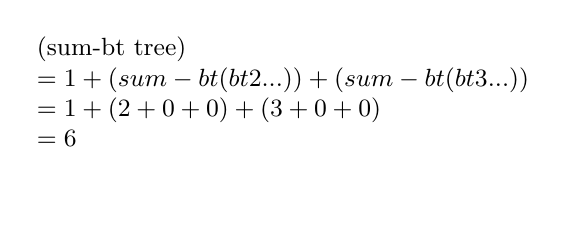
\begin{tikzpicture}[baseline=-14mm]
  \node[draw=none, fill=none, align=left, font=\small] {
    \code{(sum-bt tree)}\\
    $= 1 + \code{(sum-bt (bt 2 ...))} + \code{(sum-bt (bt 3 ...))}$\\
    $= 1 + (2 + 0 + 0) + (3 + 0 + 0)$\\
    $= 6$};
\end{tikzpicture}
\caption{The value \code{tree}. Each \code{bt} node causes two recursive calls, one per subtree.}
\label{fig:bt}
\end{figure}

Tree recursion is usually not made tail-recursive: with two recursive calls, at most one of them can be the last thing the function does, and the other has to be remembered.

\subsection{\texttt{match}}

\code{match} checks the shape and extracts the fields in one step, which reads better once all the fields are needed anyway:
\begin{lstlisting}
(define (sum-bt/match t)
  (match t
    ['() 0]
    [(bt label left right)
     (+ label (sum-bt/match left) (sum-bt/match right))]))
\end{lstlisting}
The pattern \rkt|(bt label left right)| matches only \code{bt} values and binds the three names to the fields in order.

\subsection{(SUPPLEMENT) Further Topics}

\subsubsection{Structural recursion} Functions like \code{sum-bt} are \emph{structurally recursive}: they recur only on immediate sub-parts of their input. Such functions always terminate on finite data, since each call is on a strictly smaller value, and their correctness can be proved by \emph{structural induction}, one case per variant. Every interpreter in this course is structurally recursive in its \code{eval} on the abstract syntax tree, except where substitution builds a new tree (\Cref{ch:week4}).

\subsubsection{Opaque structs and abstraction} Opacity is the default for a reason: an opaque struct hides its representation, so a module can export the struct without letting clients inspect or compare its insides. Transparent structs are the right choice for plain data such as trees and syntax, where structural equality is what you want. A middle ground is \code{\#:prefab}, which also makes structs readable and writable as literals.

\subsubsection{Contracts on fields} Plain Racket can check field types at run time with \code{struct/contract} or \code{contract-out}, e.g.\ requiring \code{left} to satisfy \code{(or/c empty? bt?)}. The error then points at the bad construction rather than the later traversal. \code{plai-typed} (\Cref{ch:week3}) instead checks before the program runs.

\section{Higher-Order Functions}
\label{sec:hof}

\subsection{Functions Are Values}

A function does not need a name. \code{lambda} builds one on the spot, and it can be called immediately: \rkt|((lambda (x) (* x x)) 4)| is \code{16}. So \code{define} for functions is shorthand, and these two definitions are the same:
\begin{lstlisting}
(define (square x)
  (* x x))

(define square-alt
  (lambda (x) (* x x)))
\end{lstlisting}
Use the short form. Do not nest one form inside the other: \rkt|(define (f x) (lambda ...))| defines a function that \emph{returns} a function, which is a different thing.

Since functions are values, a function can return one:
\begin{lstlisting}
(define (make-adder x)
  (lambda (y) (+ x y)))

(define add2 (make-adder 2))
\end{lstlisting}

\begin{definition}[Closure]
A \emph{closure} is a function value together with the bindings of the variables it refers to from the surrounding code.
\end{definition}

\rkt|(make-adder 2)| returns a function that has not been called yet but already remembers that \code{x} is 2. Then \rkt|(add2 5)| is 7, and \rkt|((make-adder 3) 4)| is 7 as well.

\subsection{\texttt{map} and \texttt{filter}}

Once functions can be arguments, the two most common list patterns become ordinary functions. \code{map} applies a function to every element; the result has the same length as the input.
\begin{lstlisting}
(define (my-map f l)
  (cond
    [(empty? l) '()]
    [else (cons (f (first l)) (my-map f (rest l)))]))
\end{lstlisting}
So
\begin{lstlisting}
(map f (list a b c))                       ; = (list (f a) (f b) (f c))
(map (lambda (x) (+ 1 x)) (list 1 2 3))    ; = '(2 3 4)
\end{lstlisting}

\code{filter} keeps the elements that pass a test; the contents are unchanged, only the length shrinks. To drop an element, return the filtered rest without \code{cons}ing it back on:
\begin{lstlisting}
(define (my-filter f l)
  (cond
    [(empty? l) '()]
    [else (if (f (first l))
              (cons (first l) (my-filter f (rest l)))
              (my-filter f (rest l)))]))
\end{lstlisting}
\rkt|(filter odd? (list 1 2 3 4 5))| is \code{'(1 3 5)}.

\begin{keypoint}[Three shapes of list code]
\code{map}: list to list, same length. \code{filter}: list to list, shorter. \code{fold}: list to a single value. Most list code is a combination of these three.
\end{keypoint}

\subsection{Folds}

\code{map} and \code{filter} each fix what happens at every step. A \emph{fold} takes the step as an argument: a two-argument \code{combine}, a \code{base} value for the empty list, and the list. It walks the list once and collapses it into one value. There are two folds, and they differ in which way the parentheses group (\Cref{fig:folds}):
\begin{align*}
\code{(my-foldl - 0 '(1 2 3))} &= ((0 - 1) - 2) - 3 = -6, \\
\code{(my-foldr - 0 '(1 2 3))} &= 1 - (2 - (3 - 0)) = 2.
\end{align*}
With an associative and commutative \code{combine} such as \code{+}, \code{*}, or \code{max}, the two agree, which is why the difference is easy to miss until it bites.

\begin{figure}[htbp]
\centering
\begin{tikzpicture}[level distance=9mm, sibling distance=9mm, every node/.style={ast}]
  \node[asth] {-}
    child {node[asth] {-}
      child {node[asth] {-} child {node[astl] {0}} child {node {1}}}
      child {node {2}}}
    child {node {3}};
  \node[draw=none, fill=none, font=\small] at (0,-4.0) {\code{foldl}: $((0-1)-2)-3$};
\end{tikzpicture}
\hspace{2cm}
\begin{tikzpicture}[level distance=9mm, sibling distance=9mm, every node/.style={ast}]
  \node[asth] {-}
    child {node {1}}
    child {node[asth] {-}
      child {node {2}}
      child {node[asth] {-} child {node {3}} child {node[astl] {0}}}};
  \node[draw=none, fill=none, font=\small] at (0,-4.0) {\code{foldr}: $1-(2-(3-0))$};
\end{tikzpicture}
\caption{The two folds of \code{-} over \code{'(1 2 3)} with base 0 (green). \code{foldl} leans left, starting from the base; \code{foldr} leans right, ending at the base.}
\label{fig:folds}
\end{figure}

\subsubsection{\code{foldl} combines on the way down} In \code{my-foldl}, \code{base} doubles as the running accumulator. Each step folds one more element into it and calls itself, and that call is a tail call, so this is a loop in constant stack space:
\begin{lstlisting}
(define (my-foldl combine base l)
  (cond
    [(empty? l) base]
    [else (my-foldl combine (combine base (first l)) (rest l))]))
\end{lstlisting}
\begin{lstlisting}[style=repl]
(my-foldl + 0 '(1 2 3 4 5))
---> (my-foldl + 1 '(2 3 4 5))
---> (my-foldl + (+ 1 2) '(3 4 5))
---> (my-foldl + (+ 3 3) '(4 5))
---> (my-foldl + (+ 6 4) '(5))
---> (my-foldl + 15 empty)
---> 15
\end{lstlisting}
Nothing is pending; at every step the accumulator is a value and the list is shorter.

\subsubsection{\code{foldr} combines on the way back up} In \code{my-foldr}, \code{combine} wraps the recursive call. No arithmetic can happen until the recursion reaches \code{'()} and the base value comes back:
\begin{lstlisting}
(define (my-foldr combine base l)
  (cond
    [(empty? l) base]
    [else (combine (first l) (my-foldr combine base (rest l)))]))
\end{lstlisting}
\begin{lstlisting}[style=repl]
(my-foldr + 0 '(1 2 3 4 5))
---> (+ 1 (my-foldr + 0 '(2 3 4 5)))
---> (+ 1 (+ 2 (my-foldr + 0 '(3 4 5))))
---> (+ 1 (+ 2 (+ 3 (+ 4 (+ 5 (my-foldr + 0 empty))))))
---> (+ 1 (+ 2 (+ 3 (+ 4 (+ 5 0)))))
---> 15
\end{lstlisting}
That growing pile of pending additions \emph{is} the stack: it is the concrete reason \code{foldr} uses $O(n)$ space and \code{foldl} $O(1)$.

\begin{keypoint}[\code{foldr} rebuilds structure]
\rkt|(my-foldr cons '() l)| copies \code{l}, because \code{foldr} replaces each \code{cons} of the list by \code{combine} and the final \code{'()} by \code{base}. Hence \code{map} and \code{filter} are both folds in disguise:
\begin{lstlisting}
(define (map-as-fold f l)
  (my-foldr (lambda (x acc) (cons (f x) acc)) '() l))

(define (filter-as-fold f l)
  (my-foldr (lambda (x acc) (if (f x) (cons x acc) acc)) '() l))
\end{lstlisting}
\end{keypoint}

\begin{pitfall}[Racket's \code{foldl} argument order]
The \code{combine} of \code{my-foldl} takes \code{(acc elem)}. Racket's built-in \code{foldl} calls \code{(combine elem acc)}, element first, the opposite order. So \rkt|(foldl - 0 '(1 2 3))| in Racket is $3-(2-(1-0)) = 2$, not $-6$. Check the order before reusing a \code{combine}.
\end{pitfall}

\section{Scope and State}
\label{sec:scopestate}

\subsection{\texttt{let} and \texttt{let*}}

\code{let} binds names to values for the extent of its body. The clauses go in one pair of brackets; square and round brackets are interchangeable in Racket, so both of these are the same form:
\begin{lstlisting}
(let ([x (+ 1 2)])
  (+ x x))            ; 6

(let [(x (+ 1 2))
      (y (+ 4 5))]
  (+ x y))            ; 12
\end{lstlisting}

The catch is \emph{when} each name starts to exist. \code{let} evaluates all of its right-hand sides first, in the scope \emph{outside} the \code{let}, and only then binds the names. So a later clause cannot use an earlier one:
\begin{lstlisting}
(let ([x (+ 1 2)]
      [y (+ 1 x)])     ; x is not bound here
  (+ x y))
;; x: undefined; cannot reference an identifier before its definition
\end{lstlisting}
Read the message as ``that name is not in scope here''.

\code{let*} binds the clauses one at a time, each in the scope of the previous ones, so this version works and gives 7:
\begin{lstlisting}
(define let-example
  (let* ([x (+ 1 2)]
         [y (+ 1 x)])
    (+ x y)))
\end{lstlisting}
There is no magic in \code{let*}; it is nested \code{let}s:
\[
\code{(let* ([x a] [y b]) body)} \quad\text{means}\quad \code{(let ([x a]) (let ([y b]) body))}.
\]
Use \code{let} by default, since it tells the reader the bindings are independent, and \code{let*} only when a clause really needs the one above it. Neither lets a clause refer to \emph{itself}: a local recursive function needs \code{letrec}, or the named \code{let} of \Cref{sec:listsrec}.

\subsection{Lexical Scope}

A \code{let} is an expression, so it can appear anywhere a value can, including in another \code{let}'s right-hand side:
\begin{lstlisting}
(define nested-let-example
  (let ([x (let ([y 3]) (+ y y))])
    (+ x x)))           ; x = 6, so 12
\end{lstlisting}
But \code{y} exists only inside the inner \code{let}. Writing \rkt|(+ x y)| in the outer body is the same undefined-identifier error, even though \code{y} was ``used'' a moment earlier (\Cref{fig:scope}).

\begin{figure}[htbp]
\centering
\begin{tikzpicture}[tok/.style={inner sep=1.5pt, font=\ttfamily\normalsize, anchor=base west}]
  \node[tok] (a1) at (0,0) {(let ([x};
  \node[tok, right=1mm of a1.base east, anchor=base west, draw, fill=uspace, rounded corners=2pt, inner sep=3pt] (inner) {(let ([y 3]) (+ y y))};
  \node[tok, right=0pt of inner.base east, anchor=base west] (a2) {])};
  \node[tok] (b1) at (0.6,-0.9) {(+ x};
  \node[tok, right=0pt of b1.base east, anchor=base west, text=sigc] (y) {\,y};
  \node[tok, right=0pt of y.base east, anchor=base west] (b2) {))};
  \begin{scope}[on background layer]
    \node[draw, fill=kspace!50, rounded corners=3pt, fit=(a1)(inner)(a2)(b2), inner sep=6pt] (outer) {};
  \end{scope}
  \node[lbl, right=3mm of a2] {scope of \code{y}: the green box};
  \node[lbl, right=3mm of b2, align=left] {scope of \code{x}: the body;\\ \code{y} is \emph{not} visible here};
\end{tikzpicture}
\caption{Scopes nest like the text. The body of the outer \code{let} is outside the inner \code{let}, so \code{y} is unbound there.}
\label{fig:scope}
\end{figure}

\begin{definition}[Lexical scope]
Under \emph{lexical} (static) scope, which binding a use of a name refers to is determined by where the binding is \emph{written} in the program text, not by what happened to run before.
\end{definition}

This is the same rule that makes the closure in \code{make-adder} work: the \code{x} in \code{(lambda (y) (+ x y))} refers to the \code{x} of the enclosing \code{define}, wherever the returned function is later called.

\subsection{Pure Code and Side Effects}

Everything so far is \emph{pure}: a call depends only on its arguments and does nothing but return a value. Run the same expression twice and you get the same answer, so an expression can always be replaced by its value without changing the program. That is what makes the step-by-step traces of \code{rev} and the folds valid reasoning, not just illustration.

A \emph{side effect} is anything else a call does: printing, mutating a variable, reading input, raising an error. In a language built on statements, \code{i++} is exactly this. Running it twice is not the same as running it once, so it cannot be replaced by its value.
\begin{itemize}
  \item \code{"Hello World"} is a value. Evaluating it does nothing else.
  \item \rkt|(print "Hello World")| writes to the console and returns \code{(void)}. The output is the point; the return value is not.
\end{itemize}
Racket does not forbid effects; it makes them ordinary expressions, so staying pure is a choice made function by function.

\subsubsection{Sequencing} A function body may hold several expressions. They run in order, the earlier ones only for their effects, and the value of the \emph{last} one is returned:
\begin{lstlisting}
(define (foo x)
  (print "Hello")
  (+ x 1))
\end{lstlisting}
\rkt|(foo 1)| returns 2 and prints along the way. The returned number is perfectly predictable; the printing is what makes \code{foo} impure. \code{begin} is the same sequencing as a single expression, for places where only one expression is allowed, such as a \code{cond} branch or an arm of \code{if}:
\begin{lstlisting}
(begin
  (print "Hello")
  (print "World")
  (+ 1 2))          ; returns 3, after printing
\end{lstlisting}

\subsubsection{Three ways to print} All return \code{(void)}; they differ only in what appears on the console. \rkt|(print "Hello")| shows \code{"Hello"}, the value as Racket would write it, quotes included. \rkt|(display "Hello")| shows \code{Hello}, the human-readable form. \rkt|(printf "The number foo is: ~a !" (* 3 3))| shows \code{The number foo is: 9 !}: \code{\textasciitilde a} splices in the display form of the next argument.

\subsection{Boxes: State You Can See}

A \emph{box} is a mutable container with exactly one slot, the smallest possible piece of state. It is a value like any other, so it can be passed to a function that changes it.
\begin{lstlisting}
(define bar (box 3))

(define (increment-box b)
  (set-box! b (+ 1 (unbox b))))
\end{lstlisting}
\rkt|(box 3)| makes a box, \rkt|(unbox bar)| reads it, and \rkt|(set-box! bar 10)| overwrites it and returns \code{(void)}. \code{increment-box} is called for its effect and returns nothing useful, so the caller has to \code{unbox} afterwards to see the new contents:
\begin{lstlisting}
(let ([b (box 3)])
  (increment-box b)
  (unbox b))          ; 4
\end{lstlisting}

The point of a box is that mutability is \emph{visible}. A plain 3 can never change; a box holding 3 announces that someone may change it, so a reader can tell where the state lives. By convention, a name ending in \code{!} mutates something: a warning that calling it twice is not the same as calling it once.

\section{Recitation 2: Boolean Expressions}
\label{sec:rec2}

This recitation builds the course's first interpreter and first program transformation, for a tiny language of Boolean expressions. Everything is in plain Racket, with structs and \code{match}.

\subsection{The Language and Its Representation}

The grammar of \emph{bexp}:
\[
\langle\textit{bexp}\rangle \;::=\; \langle\textit{boolean}\rangle \;\mid\; \langle\textit{bexp}\rangle \land \langle\textit{bexp}\rangle \;\mid\; \langle\textit{bexp}\rangle \lor \langle\textit{bexp}\rangle \;\mid\; \neg \langle\textit{bexp}\rangle
\]
One struct per alternative of the grammar represents it in Racket:
\begin{lstlisting}
(struct leaf-node (arg))
(struct or-node (left right))
(struct and-node (left right))
(struct not-node (arg))

(define bexp-bool-1 (and-node (leaf-node #t) (leaf-node #f)))
(define bexp-sym-1 (and-node (leaf-node 'x) (leaf-node 'y)))
\end{lstlisting}
A value built from these structs is an \emph{abstract syntax tree}: the tree structure replaces parentheses and precedence. Note that the structs are \emph{not} transparent and their fields are unchecked: \code{bexp-sym-1} has symbols, not booleans, at its leaves, and Racket accepts it.

\begin{exercise}[Syntactic equality]
Write \code{syn-equal?}, which checks whether two bexps are the same tree.
\end{exercise}
\begin{solution}
Because the structs are opaque, \code{equal?} would compare them by identity (\Cref{sec:structs}), so we write structural equality ourselves. \code{match*} matches several values at once, one pattern per value:
\begin{lstlisting}
(define (syn-equal? b1 b2)
  (match* (b1 b2)
    [((and-node l1 r1) (and-node l2 r2)) (and (syn-equal? l1 l2) (syn-equal? r1 r2))]
    [((or-node l1 r1) (or-node l2 r2))   (and (syn-equal? l1 l2) (syn-equal? r1 r2))]
    [((not-node a1) (not-node a2))       (syn-equal? a1 a2)]
    [((leaf-node v1) (leaf-node v2))     (equal? v1 v2)]
    [(_ _) #f]))
\end{lstlisting}
One clause per variant where both sides agree, and a final catch-all for mismatched shapes.
\end{solution}

\begin{pitfall}[A missing variant hides behind a catch-all]
If the \code{not-node} clause were left out, two \code{not-node}s would fall through to \rkt|[(_ _) #f]|, and \code{syn-equal?} would say a negation is not equal to itself. Nothing would complain, and every later test comparing expressions with a negation would fail even with a correct optimizer. With a catch-all clause present, check the list of variants, not just the clauses you were given.
\end{pitfall}

\subsection{An Interpreter for bexp}

\begin{exercise}[Interpreter]
Write \code{evaluate-bexp}, which computes the Boolean value an expression represents.
\end{exercise}
\begin{solution}
One clause per variant, and a recursive call wherever a variant contains a sub-expression:
\begin{lstlisting}
(define (evaluate-bexp b)
  (match b
    [(leaf-node v)    v]
    [(or-node b1 b2)  (or (evaluate-bexp b1) (evaluate-bexp b2))]
    [(and-node b1 b2) (and (evaluate-bexp b1) (evaluate-bexp b2))]
    [(not-node b1)    (not (evaluate-bexp b1))]))

(check-expect (evaluate-bexp (leaf-node #t)) #t)
(check-expect (evaluate-bexp (and-node (leaf-node #t) (leaf-node #f))) #f)
(check-expect (evaluate-bexp (and-node (leaf-node #f) (leaf-node #t))) #f)
\end{lstlisting}
The third test swaps the arguments of the second; testing both orders is cheap and catches an implementation that looks at only one side.
\end{solution}

This is the pattern of every interpreter in the course: our language's $\land$ is implemented by Racket's \code{and}, its $\lor$ by \code{or}, its $\neg$ by \code{not}. The \emph{meaning} of each construct is given by the clause that handles it.

\subsubsection{Missing cases} What happens with an incomplete \code{match}?
\begin{lstlisting}
(define (evaluate-bexp-m b)
  (match b
    [(leaf-node v) v]))
\end{lstlisting}
Nothing complains when it is defined. The error appears only when it is called on a value that no clause matches: \rkt|(evaluate-bexp-m bexp-bool-1)| raises \code{match: no matching clause}. Racket checks patterns at run time, so a missing case is found only if some test happens to reach it. \Cref{sec:rec3} redoes this in \code{plai-typed}, where the same mistake is rejected before the program runs.

\subsection{An Optimization Pass: De Morgan}

De Morgan's laws and double-negation elimination state the equivalences
\[
\neg(P \land Q) = \neg P \lor \neg Q, \qquad \neg(P \lor Q) = \neg P \land \neg Q, \qquad \neg\neg P = P.
\]
Using them left to right, an optimizer can eliminate redundant negations and push every remaining negation down to the leaves. The examples use symbolic leaves:
\begin{center}
\begin{tabular}{@{}lll@{}}
\toprule
name & before & after \\
\midrule
\code{bexp-1} & $\neg(\neg P \lor Q)$ & $P \land \neg Q$ \\
\code{bexp-2} & $\neg\neg P \lor \neg Q$ & $P \lor \neg Q$ \\
\code{bexp-3} & $P \lor \neg Q$ & $P \lor \neg Q$ (already optimal) \\
\bottomrule
\end{tabular}
\end{center}
\begin{lstlisting}
(define bexp-1 (not-node (or-node (not-node (leaf-node 'P)) (leaf-node 'Q))))
(define bexp-2 (or-node (not-node (not-node (leaf-node 'P))) (not-node (leaf-node 'Q))))
(define bexp-3 (or-node (leaf-node 'P) (not-node (leaf-node 'Q))))

(define bexp-1-opt (and-node (leaf-node 'P) (not-node (leaf-node 'Q))))
(define bexp-2-opt (or-node (leaf-node 'P) (not-node (leaf-node 'Q))))
(define bexp-3-opt (or-node (leaf-node 'P) (not-node (leaf-node 'Q))))
\end{lstlisting}

\subsubsection{What does it mean for an optimization to be correct?} Before writing the optimizer, decide how to check it. An optimization is correct when it does two things:
\begin{enumerate}
  \item it \emph{preserves semantics}: the output evaluates to the same value as the input;
  \item it actually \emph{optimizes}: the output has the promised shape, here every negation sitting directly on a leaf.
\end{enumerate}
Both become executable checks:
\begin{lstlisting}
(define (preserves-sem? unopt)
  (equal? (evaluate-bexp unopt) (evaluate-bexp (demorgan-opt unopt))))

(define (is-optimizing? opt)
  (define (only-not-at-leaves? bexp)
    (match bexp
      [(leaf-node v) #t]
      [(or-node b1 b2) (and (only-not-at-leaves? b1) (only-not-at-leaves? b2))]
      [(and-node b1 b2) (and (only-not-at-leaves? b1) (only-not-at-leaves? b2))]
      [(not-node (leaf-node v)) #t]
      [(not-node _) #f]))
  (only-not-at-leaves? opt))

(define (is-correct? unopt)
  (and (preserves-sem? unopt) (is-optimizing? (demorgan-opt unopt))))
\end{lstlisting}
\code{is-optimizing?} relies on \code{match} trying clauses in order: \rkt|(not-node (leaf-node v))| is tried first, so the catch-all \rkt|(not-node _)| sees only negations of compound expressions, which mean the pass left work undone. Note also that \code{preserves-sem?} takes only the input and calls \code{demorgan-opt} itself, so it tests the optimizer rather than a hand-written answer.

\subsubsection{The optimizer} What to do with a negation depends entirely on what is \emph{inside} it, so a single \rkt|(not-node b1)| clause cannot work. Nested patterns split it into the four shapes the argument can have, one per variant. This is what the handout means by ``you will need more cases than in \code{evaluate-bexp}'':
\begin{lstlisting}
(define (demorgan-opt b)
  (match b
    ; Standard Stuff
    [(leaf-node v)    (leaf-node v)]
    [(or-node b1 b2)  (or-node (demorgan-opt b1) (demorgan-opt b2))]
    [(and-node b1 b2) (and-node (demorgan-opt b1) (demorgan-opt b2))]
    [(not-node (leaf-node l)) (not-node (leaf-node l))]
    ; De-Morgan Stuff
    [(not-node (and-node b1 b2))
     (or-node (demorgan-opt (not-node b1)) (demorgan-opt (not-node b2)))]
    [(not-node (or-node b1 b2))
     (and-node (demorgan-opt (not-node b1)) (demorgan-opt (not-node b2)))]
    [(not-node (not-node b1)) (demorgan-opt b1)]))
\end{lstlisting}
\begin{itemize}
  \item \textbf{A negated leaf} is already as far down as a negation can go; keep it.
  \item \textbf{De Morgan.} After rewriting $\neg(b_1 \land b_2)$ to $\neg b_1 \lor \neg b_2$, the new negations may themselves sit on top of an \code{and}, an \code{or}, or a \code{not}, so they are optimized again: the recursive calls are on \rkt|(not-node b1)|, not on \code{b1}. Calling \rkt|(demorgan-opt b1)| would drop the negation and change the meaning.
  \item \textbf{Double negation.} The two negations cancel, and the result is \rkt|(demorgan-opt b1)|, not just \code{b1}, because \code{b1} may still contain negations to push down.
\end{itemize}

\begin{figure}[htbp]
\centering
\begin{tikzpicture}[level distance=9mm, sibling distance=14mm, every node/.style={ast}]
  \node[asth] {not}
    child {node {or}
      child {node[asth] {not} child {node[astl] {P}}}
      child {node[astl] {Q}}};
  \node[draw=none, fill=none, font=\small] at (0,-3.6) {$\neg(\neg P \lor Q)$};
\end{tikzpicture}
\hspace{0.8cm}
\begin{tikzpicture}
  \draw[arr] (0,0) -- (1.6,0) node[midway, above, lbl] {\code{demorgan-opt}};
  \node at (0,-1.6) {};
\end{tikzpicture}
\hspace{0.8cm}
\begin{tikzpicture}[level distance=9mm, sibling distance=14mm, every node/.style={ast}]
  \node {and}
    child {node[astl] {P}}
    child {node[asth] {not} child {node[astl] {Q}}};
  \node[draw=none, fill=none, font=\small] at (0,-3.6) {$P \land \neg Q$};
\end{tikzpicture}
\caption{\code{bexp-1} before and after the pass. Negations (yellow) end up only directly above leaves.}
\label{fig:demorgan}
\end{figure}

For \code{bexp-1} (\Cref{fig:demorgan}):
\begin{lstlisting}[style=repl]
(demorgan-opt (not (or (not P) Q)))
---> (and-node (demorgan-opt (not (not P))) (demorgan-opt (not Q)))   ; not over or
---> (and-node (demorgan-opt P) (not Q))                              ; not-not cancels
---> (and-node P (not Q))
\end{lstlisting}

\subsubsection{Why it terminates} Every recursive call is on a smaller tree. In the De Morgan cases the argument \rkt|(not-node b1)| is new, but it is smaller than the input \rkt|(not-node (and-node b1 b2))|, which has one more node and all of \code{b2} besides.

\subsection{Testing the Optimizer Two Ways}

The syntactic tests compare against the exact trees written by hand:
\begin{lstlisting}
(check-expect (syn-equal? (demorgan-opt bexp-1) bexp-1-opt) #t)
(check-expect (syn-equal? (demorgan-opt bexp-2) bexp-2-opt) #t)
(check-expect (syn-equal? (demorgan-opt bexp-3) bexp-3-opt) #t)
\end{lstlisting}
The semantic tests check the two correctness properties without writing the expected tree at all:
\begin{lstlisting}
(define bexp-4 (not-node (or-node (not-node (leaf-node #t)) (leaf-node #f))))
(define bexp-5 (or-node (not-node (not-node (leaf-node #t))) (not-node (leaf-node #f))))
(define bexp-6 (or-node (leaf-node #t) (not-node (leaf-node #t))))
(check-expect (is-correct? bexp-4) #t)
(check-expect (is-correct? bexp-5) #t)
(check-expect (is-correct? bexp-6) #t)
\end{lstlisting}

\begin{remark}[Why booleans at the leaves]
\code{bexp-4} to \code{bexp-6} are \code{bexp-1} to \code{bexp-3} with \code{\#t} and \code{\#f} in place of \code{'P} and \code{'Q}. With symbols at the leaves, \code{evaluate-bexp} is meaningless: \rkt|(not 'P)| is \code{\#f} and \rkt|(or 'P #f)| is \code{'P}, because Racket treats every value except \code{\#f} as true. So a semantic check only means something on Boolean leaves.
\end{remark}

\begin{remark}[The handout's table]
An earlier version of the handout listed $\neg(\neg P \land Q) \mapsto P \land Q$ as the first example. That contradicts both the code (\code{bexp-1} is built with \code{or-node}) and De Morgan's law; the posted solution corrects the row to $\neg(\neg P \lor Q) \mapsto P \land \neg Q$. Trust the definitions over the prose, and check the prose by working one example by hand.
\end{remark}


\chapter{Week 3: Types and a First Interpreter}
\label{ch:week3}

Lecture 3: September 22, 2026. Recitation 3: September 25, 2026.

Supplementary reading:
\begin{itemize}
  \item \cite{PLAI} Chapters 2 (Everything (We Will Say) About Parsing) and 3 (A First Look at Interpretation).
  \item \cite{PLAI} Chapter 15 (Checking Program Invariants Statically: Types), first sections, and the \code{plai-typed} documentation.
  \item \cite{TAPL} Chapter 1 (what type systems are for), optional.
\end{itemize}

From this week on, code is written in \code{\#lang plai-typed}, the language of the textbook: Racket with a type checker that reads the whole program before anything runs. Lecture~3 introduces its types, defines new types with \code{define-type}, and uses them to write the first interpreter of the course, a calculator. Recitation~3 redoes Recitation~2 with types and then studies Racket's \code{match} in more depth. This chapter covers:
\begin{itemize}
  \item \Cref{sec:types}: types, type inference and annotations, function types, homogeneous lists, pairs, and polymorphism;
  \item \Cref{sec:definetype}: \code{define-type}, \code{type-case}, and exhaustiveness checking;
  \item \Cref{sec:calc}: quote and s-expressions, concrete vs.\ abstract syntax, and the calculator's parser and interpreter;
  \item \Cref{sec:rec3}: Recitation~3, typed Boolean expressions and pattern matching with \code{match}.
\end{itemize}

\section{Types in plai-typed}
\label{sec:types}

\code{plai-typed} is installed with \code{raco pkg install plai-typed}, and a file starts with \code{\#lang plai-typed}. It looks like Racket, but a type checker reads the whole program first, and a program that fails the check does not run at all.

\subsection{Every Value Has a Type}

At the REPL, every answer comes with two lines: the type the checker worked out, starting with \code{-}, and then the value.
\begin{lstlisting}[style=repl]
> 3
- number
3
> (+ 3 4)
- number
7
> "hello"
- string
"hello"
> (+ 3 "hello")
typecheck failed: number vs. string
\end{lstlisting}
This is the idea of the lecture in miniature: the type is known \emph{before} the value is computed. The checker does not run \rkt|(+ 3 4)| to find out it is a number; it knows because \code{+} takes numbers and returns a number.

\subsection{Type Inference and Annotations}

No types need to be written. Here the checker sees \rkt|(+ 3 x)|, concludes that \code{x} must be a number, and that the result is one too:
\begin{lstlisting}
(define (add3 x)
  (+ 3 x))
\end{lstlisting}

\begin{definition}[Type inference]
\emph{Type inference} is the checker working out the types that the programmer did not write down.
\end{definition}

Types can also be written, as many or as few as we like. An argument becomes \rkt|(x : number)|, and the return type goes after the argument list. Whatever is left out is inferred:
\begin{lstlisting}
(define (add3-v2 (x : number))            ; return type inferred
  (+ 3 x))

(define (add3-v3 (x : number)) : number   ; both annotated
  (+ 3 x))
\end{lstlisting}

\begin{pitfall}[Spaces around the colon]
\code{(x: number)} is read as one identifier named \code{x:}, followed by \code{number}, and is rejected with \code{expected either <id> or `[<id> : <type>]'}. Write \code{(x : number)}.
\end{pitfall}

An annotation is a claim the checker verifies, not a hint it trusts. This one is wrong, since \rkt|(+ 3 x)| is a number, so the definition is rejected:
\begin{lstlisting}
(define (add3-v4 (x : number)) : string
  (+ 3 x))
;; typecheck failed: number vs. string
\end{lstlisting}
Either way the program is checked before it runs: a call like \rkt|(add3-v3 "hello")| never gets the chance to fail at run time, because the whole file is rejected.

If the checker can infer the types, why write them? Two reasons from lecture:
\begin{itemize}
  \item \textbf{Documentation.} The reader sees what the function takes and returns without reading its body.
  \item \textbf{Mental model.} Writing the type first makes you decide what the function is supposed to do before you write how it does it.
\end{itemize}

\subsection{Function Types}
\label{sec:fntypes}

Functions are values, so they have types. Read the arrow as ``takes \ldots{} and returns \ldots'':
\begin{lstlisting}[style=repl]
> add3
- (number -> number)
\end{lstlisting}
With two arguments, both go to the left of the arrow. Annotations can be mixed: in \code{myadd-v2}, \code{y} is unannotated but added to a number, so it is inferred to be one, and the two functions have the same type.
\begin{lstlisting}
(define (myadd x y)
  (+ x y))
(define (myadd-v2 (x : number) y) : number
  (+ x y))
\end{lstlisting}
\begin{lstlisting}[style=repl]
> myadd
- (number number -> number)
> myadd-v2
- (number number -> number)
\end{lstlisting}

A function that returns a function, \code{make-adder} from \Cref{sec:hof}, now has a type that says so:
\begin{lstlisting}
(define (myadd-v3 (x : number))
  (lambda (y) (+ x y)))
\end{lstlisting}
\begin{lstlisting}[style=repl]
> myadd-v3
- (number -> (number -> number))
> (myadd-v3 2)
- (number -> number)
> ((myadd-v3 2) 5)
- number
7
\end{lstlisting}
Compare the two types. \code{myadd} takes two numbers at once. \code{myadd-v3} takes \emph{one} number and returns a function that waits for the second, so \rkt|(myadd-v3 2)| is not a number yet but a function.

\subsection{Lists Are Homogeneous}

A list type says what its elements are, and every element must have that type:
\begin{lstlisting}[style=repl]
> (list 1 2 3 4)
- (listof number)
'(1 2 3 4)
> (cons 3 (cons 4 empty))
- (listof number)
'(3 4)
> (list 1 "hello")
typecheck failed: number vs. string
> (cons 3 4)
typecheck failed: (listof number) vs. number
\end{lstlisting}
Plain Racket accepts both of the last two. In \code{plai-typed} the second argument of \code{cons} must be a list, so bare pairs (\Cref{sec:lists}) are impossible. In exchange, list operations have precise types: the checker knows \rkt|(first (list 1 2 3 4))| is a \code{number} and \rkt|(rest (list 1 2 3 4))| a \code{(listof number)}, and likewise for \code{second} and \code{third}, without running anything.

\subsection{Pairs}

When two values of different types belong together, use a \emph{pair} (a tuple). Its type is written with \code{*}:
\begin{lstlisting}[style=repl]
> (pair 1 "hello")
- (number * string)
'#(1 "hello")
> (fst (pair 1 2))
- number
1
> (snd (pair 1 2))
- number
2
> (car (pair 1 2))
car: unbound identifier
\end{lstlisting}
A list has any length but one element type; a pair has exactly two slots, each with its own type. A pair is not a cons cell, and \code{plai-typed} provides no \code{car} or \code{cdr} at all: use \code{fst}/\code{snd} for pairs and \code{first}/\code{rest} for lists.

\subsection{Polymorphic Types}

Asking for the type of \code{first} shows something new:
\begin{lstlisting}[style=repl]
> first
- ((listof 'a) -> 'a)
> rest
- ((listof 'a) -> (listof 'a))
> cons
- ('a (listof 'a) -> (listof 'a))
> fst
- (('a * 'b) -> 'a)
> map
- (('a -> 'b) (listof 'a) -> (listof 'b))
\end{lstlisting}

\begin{definition}[Type variable, parametric polymorphism]
\code{'a} (read ``alpha'') is a \emph{type variable}: any type may stand in its place, but every \code{'a} in one type must stand for the \emph{same} type. A single definition that works uniformly at every type in this way is \emph{parametrically polymorphic}; other languages call it generics.
\end{definition}

So \code{first} takes a \code{(listof number)} to a \code{number} and a \code{(listof string)} to a \code{string}, but can never take a list of numbers to a string. Different letters allow different types: \code{fst} takes a pair of an \code{'a} and a \code{'b} and returns the \code{'a}. And the type of \code{map} alone says most of what \code{map} does: given a function from \code{'a} to \code{'b} and a list of \code{'a}, it produces a list of \code{'b}.

\subsection{Why Insist on Homogeneous Lists?}

Suppose \rkt|(list 1 "hello")| were allowed; call it \code{l}. What is the type of \rkt|(first l)|? It depends on which element happens to come first, and the checker cannot know that before the program runs. Then
\begin{itemize}
  \item every use of \code{first} would need a check at run time, which is exactly what a type checker is supposed to spare us, and
  \item \rkt|(map f l)| is only safe if \code{f} accepts \emph{both} numbers and strings, which \code{('a -> 'b)} cannot express.
\end{itemize}
One could design a type that lists every position, something like \code{(listof number string number)} for \rkt|(list 1 "hello" 2)|, but then every list function (\code{map}, \code{filter}, the folds) would need a far more complicated type. The simpler fix keeps lists homogeneous and instead makes \emph{one} type that covers all the kinds of things to be mixed. That is what \code{define-type} is for.

\section{\texttt{define-type} and \texttt{type-case}}
\label{sec:definetype}

\subsection{Defining a Type with Variants}

A shape is either a circle or a rectangle:
\begin{lstlisting}
(define-type Shape
  [circle (radius : number)]                       ; variant 1
  [rectangle (width : number) (height : number)])  ; variant 2
\end{lstlisting}
This defines one new type, \tyname{Shape}, with two \emph{variants}. Each variant has a constructor and typed fields:
\begin{lstlisting}[style=repl]
> (circle 3)
- Shape
(circle 3)
\end{lstlisting}
Now \rkt|(list (circle 1) (rectangle 2 3))| is fine: the elements are different kinds of shapes, but they have one type, so the list is a \code{(listof Shape)}.

Like \code{struct}, \code{define-type} also generates
\begin{itemize}
  \item predicates \code{circle?} and \code{rectangle?}, of type \code{(Shape -> boolean)}, and
  \item accessors \code{circle-radius}, \code{rectangle-width}, and \code{rectangle-height}, of type \code{(Shape -> number)}.
\end{itemize}
The predicates accept only shapes. In plain Racket \rkt|(circle? 5)| would return \code{\#f}; here it never runs:
\begin{lstlisting}[style=repl]
> (circle? 5)
typecheck failed: Shape vs. number
\end{lstlisting}

\subsubsection{A recursive type} A type may mention itself. The binary tree of \Cref{sec:structs}, now with types:
\begin{lstlisting}
(define-type Tree
  [emp]
  [node (n : number) (lt : Tree) (rt : Tree)])
\end{lstlisting}
A variant with no fields is still a constructor, so the empty tree is \rkt|(emp)|, with parentheses. \rkt|(node 3 (emp) (emp))| has type \tyname{Tree}.

\subsection{\texttt{struct} vs.\ \texttt{define-type}}

Both make compound values, but they promise different things:
\begin{center}
\begin{tabular}{@{}p{0.47\linewidth}p{0.47\linewidth}@{}}
\toprule
\code{struct} (\code{\#lang racket}) & \code{define-type} (\code{plai-typed}) \\
\midrule
one kind of value: a \code{bt} is always a \code{bt} & one \emph{type} with several variants: \code{circle} or \code{rectangle} \\
fields unchecked: \rkt|(bt 1 2 3)| is accepted, and fails later & every field typed: \rkt|(node 3 5 (emp))| is rejected before the program runs, at the line that is wrong \\
different structs cannot share a homogeneous list type & all variants fit in one \code{(listof Shape)} \\
\bottomrule
\end{tabular}
\end{center}

\subsubsection{Why only one \code{circle}?} No other type in the program may also have a variant named \code{circle}. The immediate reason is that \code{circle}, \code{circle?}, and \code{circle-radius} are ordinary definitions, so a second \code{define-type} would define them again (\code{identifier already defined}). The deeper reason is inference: when the checker sees \rkt|(circle 3)|, the constructor's name is all it has to go on. If two types both had a \code{circle} variant, \rkt|(circle 3)| could belong to either, and inference would be stuck.

\subsection{\texttt{type-case}: Taking a Value Apart}

A \code{define-type} value is built with a constructor; \code{type-case} takes it apart again. There is one clause per variant, and the names in parentheses are bound to that variant's fields, in order (the names need not match those in \code{define-type}; only the order matters):
\begin{lstlisting}
(define (area s)
  (type-case Shape s
    [circle (r) (* 3.14159 (* r r))]
    [rectangle (w h) (* w h)]))
\end{lstlisting}
\begin{lstlisting}[style=repl]
> (area (circle 3))
- number
28.27431
> area
- (Shape -> number)
\end{lstlisting}
The same function can be written with the generated predicates and accessors:
\begin{lstlisting}
(define (area-v2 s)
  (cond
    [(circle? s) (* 3.14159 (* (circle-radius s) (circle-radius s)))]
    [(rectangle? s) (* (rectangle-width s) (rectangle-height s))]))
\end{lstlisting}
It works, but \code{type-case} is shorter, names the fields, and lines the code up with the type: one clause per variant, just as list functions had one \code{cond} branch per kind of list.

\subsection{Exhaustiveness}

The real difference shows when a case is forgotten. \code{type-case} knows every variant of \tyname{Shape}, so leaving one out is rejected before the program runs:
\begin{lstlisting}
(define (area-v3 s)
  (type-case Shape s
    [circle (r) (* 3.14159 (* r r))]))
;; type-case: syntax error; probable cause: you did not include a case
;; for the rectangle variant, or no else-branch was present
\end{lstlisting}
\code{cond} knows nothing about \tyname{Shape}; it tries its tests in order. The same mistake with \code{cond} is accepted, works on circles, and fails only at run time when it meets a rectangle:
\begin{lstlisting}
(define (area-v4 s)
  (cond
    [(circle? s) (* 3.14159 (* (circle-radius s) (circle-radius s)))]))
\end{lstlisting}
\begin{lstlisting}[style=repl]
> (area-v4 (circle 1))
- number
3.14159
> (area-v4 (rectangle 2 3))
cond: no matching clause
\end{lstlisting}

\begin{keypoint}[What \code{type-case} buys]
\code{type-case} checks before the program runs that every variant is handled, and it gives each clause the variant's fields with their types. A missing case is a static error, not a bug waiting for the right input.
\end{keypoint}

\section{S-Expressions and the Calculator}
\label{sec:calc}

\subsection{Quote and Symbols}

The apostrophe \code{'}, read ``quote'', means ``do not evaluate this; keep it as data''. Without it, \code{x} is a variable to look up. With it, \code{'x} is the name itself, a \emph{symbol}:
\begin{lstlisting}[style=repl]
> x
x: free variable while typechecking in: x
> 'x
- symbol
'x
\end{lstlisting}
Quoting a parenthesized expression keeps the whole thing as data, without doing the addition:
\begin{lstlisting}[style=repl]
> '(1 (+ 2 3) 4)
- s-expression
'(1 (+ 2 3) 4)
\end{lstlisting}

\subsection{S-Expressions}

Look at what \code{'(+ 2 3)} contains: a symbol and two numbers. That is exactly the kind of mixed list that \Cref{sec:types} ruled out. So \code{plai-typed} gives all quoted data one type, \tyname{s-expression}, and provides functions to ask what a piece is and to convert it back out:
\begin{lstlisting}[style=repl]
> (s-exp->list '(+ 2 3))
- (listof s-expression)
'(+ 2 3)
> (first (s-exp->list '(+ 2 3)))
- s-expression
'+
> (s-exp->symbol (first (s-exp->list '(+ 2 3))))
- symbol
'+
> (s-exp->number (second (s-exp->list '(+ 2 3))))
- number
2
\end{lstlisting}

\begin{keypoint}[Ask, then convert]
Ask with \code{s-exp-number?}, \code{s-exp-symbol?}, or \code{s-exp-list?}, then convert with the matching \code{s-exp->number}, \code{s-exp->symbol}, or \code{s-exp->list}. A conversion fails at run time if the guess was wrong.
\end{keypoint}

\begin{pitfall}[A lone quoted symbol is not an s-expression]
\code{'x} has type \tyname{symbol}, not \tyname{s-expression}, so \code{(parse 'x)} is a type error. To get an s-expression for one symbol, write \rkt|`x| (backquote) or \rkt|(symbol->s-exp 'x)|.
\end{pitfall}

\subsection{Concrete and Abstract Syntax}

The first interpreter is a calculator:
\begin{lstlisting}[style=repl]
'(+ 2 3)                     ===> 5
'(* 3 4)                     ===> 12
'(* (+ 2 3) (* 5 (+ 6 7)))   ===> 325
\end{lstlisting}
Following \cite[Chapters~2--3]{PLAI}, the work is split into separate steps (\Cref{fig:pipeline}):
\begin{itemize}
  \item \textbf{Concrete syntax} is what the programmer types, the text \code{(+ 2 3)}. Racket's \emph{reader} already turns text into an s-expression, so we get that step for free; quote is how we hand an s-expression over directly.
  \item \textbf{Abstract syntax} is a tree that keeps only the meaning. \code{parse} turns an s-expression into this tree, rejecting anything that is not a valid program.
  \item The \textbf{interpreter} walks the tree and computes the answer. \cite{PLAI} calls it \code{interp}; in lecture it is \code{eval}.
\end{itemize}

\begin{figure}[htbp]
\centering
\begin{tikzpicture}[node distance=4mm and 14mm]
  \node[box, fill=greybg] (t) {text};
  \node[box, fill=uspace, right=of t] (s) {s-expression};
  \node[box, fill=kspace, right=of s] (a) {\tyname{ArithE}};
  \node[box, fill=tsk, right=of a] (n) {number};
  \draw[arr] (t) -- node[above, lbl] {read} (s);
  \draw[arr] (s) -- node[above, lbl] {\code{parse}} (a);
  \draw[arr] (a) -- node[above, lbl] {\code{eval}} (n);
  \node[below=2mm of t, lbl] (et) {\code{"(+ 2 3)"}};
  \node[below=2mm of s, lbl] (es) {\code{'(+ 2 3)}};
  \node[below=2mm of a, lbl, align=center] (ea) {\code{(plusC (numC 2)}\\\code{(numC 3))}};
  \node[below=2mm of n, lbl] (en) {\code{5}};
  \draw[decorate, decoration={brace, amplitude=4pt, mirror}] ([yshift=-11mm]t.south west) -- ([yshift=-11mm]s.south east) node[midway, below=5pt, lbl] {concrete syntax};
  \draw[decorate, decoration={brace, amplitude=4pt, mirror}] ([yshift=-11mm,xshift=-6mm]a.south west) -- ([yshift=-11mm,xshift=6mm]a.south east) node[midway, below=5pt, lbl] {abstract syntax};
\end{tikzpicture}
\caption{The interpreter pipeline. Racket's reader provides the first step.}
\label{fig:pipeline}
\end{figure}

\subsection{The Calculator}

\subsubsection{Abstract syntax} One variant per kind of expression:
\begin{lstlisting}
(define-type ArithE
  [numC (n : number)]
  [plusC (e1 : ArithE) (e2 : ArithE)]
  [timesC (e1 : ArithE) (e2 : ArithE)])
\end{lstlisting}
The operands of \code{plusC} are \tyname{ArithE}, not \code{number}. That is what allows \code{'(* (+ 2 3) 4)}: the left operand of the multiplication is itself an addition, the same trick as \tyname{Tree} having subtrees (\Cref{fig:calcast}).

\begin{figure}[htbp]
\centering
\begin{tikzpicture}[level distance=9mm, every node/.style={ast},
    level 1/.style={sibling distance=34mm}, level 2/.style={sibling distance=17mm}, level 3/.style={sibling distance=12mm}]
  \node[asth] {timesC}
    child {node {plusC} child {node[astl] {numC 2}} child {node[astl] {numC 3}}}
    child {node[asth] {timesC}
      child {node[astl] {numC 5}}
      child {node {plusC} child {node[astl] {numC 6}} child {node[astl] {numC 7}}}};
\end{tikzpicture}
\caption{The abstract syntax of \code{'(* (+ 2 3) (* 5 (+ 6 7)))}. Parentheses are gone; the nesting is the tree.}
\label{fig:calcast}
\end{figure}

\subsubsection{The interpreter} One clause per variant:
\begin{lstlisting}
(define (eval (e : ArithE)) : number
  (type-case ArithE e
    [numC (n) n]
    [plusC (e1 e2) (+ (eval e1) (eval e2))]
    [timesC (e1 e2) (* (eval e1) (eval e2))]))
\end{lstlisting}
Three variants, three clauses, and a recursive call wherever the type mentions \tyname{ArithE}. \code{eval} never checks whether its input makes sense, and it does not have to: a value of type \tyname{ArithE} can only be built from the three constructors, so every tree it receives is well formed.

\subsubsection{The parser} That guarantee has to come from somewhere, and it comes from \code{parse}. The version written in lecture:
\begin{lstlisting}
(define (parse (s : s-expression)) : ArithE
  (cond
    [(s-exp-number? s) (numC (s-exp->number s))]
    [(s-exp-list? s)
     (let [(l (s-exp->list s))]
       (case (s-exp->symbol (first l))
         [(+) (plusC (parse (second l)) (parse (third l)))]
         [(*) (timesC (parse (second l)) (parse (third l)))]))]))
\end{lstlisting}
A number becomes a \code{numC}. A list is dispatched on its first element with \code{case}, which compares a symbol against literal symbols, and each operand is parsed recursively. Putting the steps together, \rkt|(eval (parse '(* (+ 2 3) (* 5 (+ 6 7)))))| is 325.

\subsection{What Malformed Input Does}

The lecture parser is right on well-formed input, but on bad input it either crashes with a message about something else, or quietly builds a wrong tree:
\begin{center}
\begin{tabular}{@{}ll@{}}
\toprule
input & result \\
\midrule
\code{(parse '(- 1 2))} & \code{case: no matching clause} \\
\code{(parse '(+ 1))} & \code{third: list contains too few elements} \\
\code{(parse '(+ 1 2 3))} & \code{(plusC (numC 1) (numC 2))}: the 3 is silently dropped \\
\bottomrule
\end{tabular}
\end{center}
The last one is the worst kind of bug: no error, just a program that means something other than what was written. A more careful parser checks the shape of each form and reports what was expected. This version is not from lecture, but every check in it addresses one row of the table:
\begin{lstlisting}
(define (parse (s : s-expression)) : ArithE
  (cond
    [(s-exp-number? s) (numC (s-exp->number s))]
    [(s-exp-list? s)
     (let [(l (s-exp->list s))]
       (if (and (= (length l) 3) (s-exp-symbol? (first l)))
           (case (s-exp->symbol (first l))
             [(+) (plusC (parse (second l)) (parse (third l)))]
             [(*) (timesC (parse (second l)) (parse (third l)))]
             [else (error 'parse "unknown operator")])
           (error 'parse "expected (op e1 e2)")))]
    [else (error 'parse "expected a number or a list")]))
\end{lstlisting}
\begin{itemize}
  \item The length check rejects \code{'(+ 1)} and \code{'(+ 1 2 3)}.
  \item \code{s-exp-symbol?} rejects \code{'(1 2 3)}, whose head is not an operator at all.
  \item The \code{else} of \code{case} rejects operators the language does not have, such as \code{-}.
  \item The final \code{else} rejects anything that is neither a number nor a list, such as a lone symbol.
\end{itemize}

\subsection{(SUPPLEMENT) Further Topics}

\subsubsection{Why parsing is cheap here} Real languages need a lexer and a parser, often generated from a grammar, to get from text to a tree. Lisp-family languages put that work into one generic step: the reader turns any text into nested lists of atoms, and each language then only has to interpret those lists. \cite[Chapter~2]{PLAI} uses this to skip parsing entirely. The flip side is that the s-expression \code{'(+ 1 2 3)} is perfectly well formed as data; deciding that it is not a valid \emph{calculator} program is the job of \code{parse}.

\subsubsection{Homoiconicity and quasiquote} Racket code is itself written as s-expressions, so programs can build programs as data. Quasiquote makes that convenient: if \code{x} is 5, then \rkt|`(+ ,x 1)| is the list \code{'(+ 5 1)}. Everything is quoted except the parts marked with a comma, which are evaluated and spliced in; \code{,@xs} splices in the elements of a whole list. Racket macros are functions from syntax to syntax built on the same idea, which is a large part of why Racket is good at implementing languages.

\subsubsection{Desugaring} The calculator has no subtraction. One way to add it without touching \code{eval} is to translate it in the parser: \code{(- a b)} becomes \code{(plusC a (timesC (numC -1) b))}. Languages are usually defined as a small \emph{core} interpreted directly plus a \emph{surface} that desugars into it~\cite[Chapter~4]{PLAI}. The core stays small enough to reason about, and the surface stays convenient.

\section{Recitation 3: Typed Boolean Expressions and Pattern Matching}
\label{sec:rec3}

Recitation~3 has two halves. Part~A (handout 3a) redoes Recitation~2's interpreter and De Morgan optimizer in \code{plai-typed}, to see what the type checker buys. Part~B (handout 3b) returns to plain Racket and studies \code{match}: literal patterns, wildcards, and taking lists apart.

\subsection{Part A: Boolean Expressions, Typed}

\subsubsection{From four structs to one type} In \Cref{sec:rec2}, a Boolean expression was built from four unrelated structs; ``a bexp'' existed only in our heads, and no field had a type. With \code{define-type}, the four become variants of \emph{one} type, and every field says what it holds:
\begin{lstlisting}
(define-type bexp-b
  [leaf-node-b (b : boolean)]
  [and-node-b (b1 : bexp-b) (b2 : bexp-b)]
  [or-node-b (b1 : bexp-b) (b2 : bexp-b)]
  [not-node-b (b : bexp-b)])
\end{lstlisting}

\begin{exercise}[Typed evaluator]
Implement \code{evaluate-bexp-b} with \code{type-case}.
\end{exercise}
\begin{solution}
\code{type-case} plays the role \code{match} played last week:
\begin{lstlisting}
(define (evaluate-bexp-b [b : bexp-b]) : boolean
  (type-case bexp-b b
    [leaf-node-b (v) v]
    [and-node-b (b1 b2) (and (evaluate-bexp-b b1) (evaluate-bexp-b b2))]
    [or-node-b (b1 b2) (or (evaluate-bexp-b b1) (evaluate-bexp-b b2))]
    [not-node-b (b1) (not (evaluate-bexp-b b1))]))

(test (evaluate-bexp-b (leaf-node-b #t)) #t)
(test (evaluate-bexp-b (and-node-b (leaf-node-b #t) (leaf-node-b #f))) #f)
(test (evaluate-bexp-b (not-node-b (or-node-b (leaf-node-b #f) (leaf-node-b #f)))) #t)
\end{lstlisting}
\code{test} is \code{plai-typed}'s \code{check-expect}, and \rkt|(print-only-errors true)| at the top of the file makes passing tests silent. This is the same shape as \code{eval} for \tyname{ArithE} in \Cref{sec:calc}.
\end{solution}

\subsubsection{What do the types buy us?}
\begin{enumerate}[label=(\alph*)]
  \item \textbf{Bad leaves are rejected before anything runs.} Last week's \code{bexp-sym-1} was
\begin{lstlisting}
(and-node (leaf-node 'x) (leaf-node 'y))
\end{lstlisting}
  and \code{evaluate-bexp} happily returned \code{'y}: Racket treats every value except \code{\#f} as true, so \rkt|(and 'x 'y)| is \code{'y}. No error, just an answer of the wrong kind. The typed version
\begin{lstlisting}
(evaluate-bexp-b (and-node-b (leaf-node-b 'x) (leaf-node-b 'y)))
\end{lstlisting}
  is rejected (\code{typecheck failed: boolean vs.\ symbol}) before anything runs, and the error points at the leaf that is wrong, not at some later function that trips over it.
  \item \textbf{Missing cases are rejected too.} Last week's \code{evaluate-bexp-m} handled only leaves; it was accepted and failed only when called on something else. The typed version
\begin{lstlisting}
(define (evaluate-bexp-b-m [b : bexp-b]) : boolean
  (type-case bexp-b b
    [leaf-node-b (v) v]))
\end{lstlisting}
  stops the program from starting: \code{you did not include a case for the and-node-b variant}. This is the \code{area-v3}/\code{area-v4} contrast of \Cref{sec:definetype} again.
\end{enumerate}

\subsubsection{De Morgan, typed} Now the leaves are variables:
\begin{lstlisting}
(define-type bexp
  [leaf-node (s : symbol)]
  [and-node (b1 : bexp) (b2 : bexp)]
  [or-node (b1 : bexp) (b2 : bexp)]
  [not-node (b1 : bexp)])
\end{lstlisting}

\begin{exercise}[Port \code{demorgan-opt} to \code{plai-typed}]
Rewrite the optimizer of \Cref{sec:rec2} for the type \tyname{bexp}.
\end{exercise}
\begin{solution}
Last week's \code{match} could name a nested pattern directly, such as \rkt|(not-node (and-node b1 b2))|. A \code{type-case} clause only takes apart the \emph{outermost} constructor, so the \code{not-node} clause needs a second \code{type-case}, on the thing being negated:
\begin{lstlisting}
(define (demorgan-opt [b : bexp]) : bexp
  (type-case bexp b
    [leaf-node (v) (leaf-node v)]
    [and-node (b1 b2) (and-node (demorgan-opt b1) (demorgan-opt b2))]
    [or-node (b1 b2) (or-node (demorgan-opt b1) (demorgan-opt b2))]
    [not-node (b1)
      (type-case bexp b1
        [leaf-node (v) (not-node (leaf-node v))]
        [and-node (b2 b3) (or-node (demorgan-opt (not-node b2))
                                   (demorgan-opt (not-node b3)))]
        [or-node (b2 b3) (and-node (demorgan-opt (not-node b2))
                                   (demorgan-opt (not-node b3)))]
        [not-node (b2) (demorgan-opt b2)])]))
\end{lstlisting}
The inner clauses are the four nested patterns of last week, one per variant of the negated expression: a negated leaf stays; $\neg(b_2 \land b_3)$ becomes $\neg b_2 \lor \neg b_3$ with both new negations optimized again; $\neg(b_2 \lor b_3)$ symmetrically; and $\neg\neg b_2$ becomes the optimized $b_2$. Both \code{type-case}s are checked for exhaustiveness, so a forgotten shape of negation is now a static error.
\end{solution}

The tests no longer need \code{syn-equal?}: \code{test} compares \code{define-type} values structurally.
\begin{lstlisting}
(define bexp-1 (not-node (or-node (not-node (leaf-node 'P)) (leaf-node 'Q))))
(define bexp-2 (or-node (not-node (not-node (leaf-node 'P))) (not-node (leaf-node 'Q))))
(define bexp-3 (or-node (leaf-node 'P) (not-node (leaf-node 'Q))))

(test (demorgan-opt bexp-1) (and-node (leaf-node 'P) (not-node (leaf-node 'Q))))
(test (demorgan-opt bexp-2) (or-node (leaf-node 'P) (not-node (leaf-node 'Q))))
(test (demorgan-opt bexp-3) (or-node (leaf-node 'P) (not-node (leaf-node 'Q))))
\end{lstlisting}

\subsection{Part B: Pattern Matching with \texttt{match}}

So far \code{match} has only taken structs apart. It can also match literal values, ignore parts of the input with wildcards, and take lists apart.

\subsubsection{Matching on values} A pattern can be a literal, which makes \code{match} a compact conditional:
\begin{lstlisting}
(define (factorial x)
  (match x
    [0 1]
    [_ (* x (factorial (- x 1)))]))

(define (factorial-if x)
  (if (= x 0)
      1
      (* x (factorial-if (- x 1)))))
\end{lstlisting}
\code{\_} is the \emph{wildcard}: it matches anything and binds nothing. Clauses are tried top to bottom, so \code{\_} goes last as the catch-all. With two cases \code{match} and \code{if} are about the same size; with more, nested \code{if}s pile up:
\begin{lstlisting}
(define (fibonacci-if x)
  (if (= x 0)
      0
      (if (= x 1)
          1
          (+ (fibonacci-if (- x 1)) (fibonacci-if (- x 2))))))
\end{lstlisting}

\begin{exercise}[Fibonacci with \code{match}]
Rewrite \code{fibonacci-if} using \code{match}.
\end{exercise}
\begin{solution}
One line per case, and the structure stays flat:
\begin{lstlisting}
(define (fibonacci x)
  (match x
    [0 0]
    [1 1]
    [_ (+ (fibonacci (- x 1)) (fibonacci (- x 2)))]))

(check-expect (fibonacci 1) 1)
(check-expect (fibonacci 10) 55)
(check-expect (fibonacci 10) (fibonacci-if 10))
\end{lstlisting}
\end{solution}

\begin{exercise}[What is \code{else}?]
\code{[else ...]} often appears as the last clause of a \code{match}. Predict \rkt|(match 5 [else else])|.
\end{exercise}
\begin{solution}
It is \code{5}. Inside \code{match}, \code{else} is not a keyword but a \emph{pattern variable}, like \code{x}: it matches anything and is bound to what it matched. So here \code{else} is bound to 5 and the clause returns it. That is why \code{[else ...]} happens to work as a catch-all; but it is an accident, and it quietly binds a variable named \code{else} in the body. Use \code{\_} instead.
\end{solution}

\subsubsection{Destructuring lists} Two attempts at ``the third element of a list'':
\begin{lstlisting}
(define (my-third x)
  (match x
    [(list a b c d) c]
    [_ x]))

(define (other-third lst)
  (match lst
    [(cons _ (cons _ (cons third _))) third]
    [_ (error "List too short")]))
\end{lstlisting}

\begin{exercise}[Predict]
On which inputs do the two functions behave differently, and why?
\end{exercise}
\begin{solution}
\rkt|(list a b c d)| matches a list of \emph{exactly} four elements. \rkt|(cons _ (cons _ (cons third _)))| matches any list of \emph{at least} three: the last \code{\_} matches whatever rest is left, including \code{'()}.
\begin{center}
\begin{tabular}{@{}lll@{}}
\toprule
input & \code{my-third} & \code{other-third} \\
\midrule
\rkt|(list 2 3)| & \code{'(2 3)} & error \code{"List too short"} \\
\code{0} & \code{0} & error \\
\rkt|(list '(2 3) 2 4 5 6 7)| & the whole list & \code{4} \\
\rkt|(list 1 2 3 4)| & \code{3} & \code{3} \\
\bottomrule
\end{tabular}
\end{center}
\begin{lstlisting}
(check-expect (my-third (list 2 3)) (list 2 3))
(check-expect (my-third 0) 0)
(check-expect (my-third (list '(2 3) 2 4 5 6 7)) (list '(2 3) 2 4 5 6 7))
(check-expect (my-third (list 1 2 3 4)) 3)

(check-error (other-third (list 2 3)) "List too short")
(check-error (other-third 0) "List too short")
(check-expect (other-third (list '(2 3) 2 4 5 6 7)) 4)
(check-expect (other-third (list 1 2 3 4)) 3)
\end{lstlisting}
\code{my-third} is right only on four-element lists, and when it is wrong it does not fail: the fallback \rkt|[_ x]| hands back its input, so the caller gets a list or a number where it expected the third element. That is the same kind of silent wrong answer as the calculator parser turning \code{'(+ 1 2 3)} into $1 + 2$ (\Cref{sec:calc}). Raising an error, as \code{other-third} does, is better.
\end{solution}

\begin{exercise}[Fix \code{my-third}]
Make \code{my-third} return the third element of any list with at least three elements and raise an error otherwise, using a \code{list} pattern. Hint: \code{\_ ...} matches zero or more elements.
\end{exercise}
\begin{solution}
\begin{lstlisting}
(define (my-third-fixed x)
  (match x
    [(list _ _ c _ ...) c]
    [_ (error "List too short")]))

(check-error (my-third-fixed (list 2 3)) "List too short")
(check-expect (my-third-fixed (list 1 2 3)) 3)
(check-expect (my-third-fixed (list '(2 3) 2 4 5 6 7)) 4)
\end{lstlisting}
This is equivalent to \code{other-third}'s nested \code{cons} pattern, and easier to read.
\end{solution}

\subsection{\texttt{match} vs.\ \texttt{type-case}}

The two halves used two tools for taking values apart. Each is strong where the other is weak:
\begin{center}
\begin{tabular}{@{}lll@{}}
\toprule
 & \code{match} & \code{type-case} \\
\midrule
language & \code{racket} & \code{plai-typed} \\
nested patterns & yes: \rkt|(not-node (and-node b1 b2))| & no: one level; nest another \code{type-case} \\
literals, wildcards, lists & yes & no \\
missing case & run-time error, only if reached & rejected before the program runs \\
\bottomrule
\end{tabular}
\end{center}
\code{match} is more expressive. \code{type-case} is more limited, and in exchange it can check, before anything runs, that every variant is handled. Recitation~4 (\Cref{sec:rec4}) implements a small \code{match} in our own interpreter.

\subsection{(SUPPLEMENT) Further Topics}

\subsubsection{More \code{match} patterns} Racket's \code{match} has many more pattern forms~\cite[Section~12]{RacketGuide}: \rkt|(? even? n)| matches when the predicate holds and binds \code{n}; \rkt|(and p1 p2)| and \rkt|(or p1 p2)| combine patterns; \rkt|(list-rest a b rest)| names the tail; \rkt|(app f p)| matches \code{p} against \rkt|(f v)|; and a clause can carry a guard with \code{\#:when}. Repeating a pattern variable, as in \rkt|(list x x)|, requires the two parts to be \code{equal?}.

\subsubsection{Exhaustiveness for richer patterns} Languages with both nested patterns and types, such as OCaml, Haskell, and Rust, get the best of both columns of the table: the compiler checks a set of nested patterns for exhaustiveness and also warns about \emph{redundant} clauses that can never match (like a clause after \code{\_}). The check is done by computing which values are not yet covered, clause by clause, and it is the same algorithm a compiler uses to turn a \code{match} into an efficient decision tree.


\chapter{Week 4: Names and Functions}
\label{ch:week4}

Lecture 4: September 29, 2026. Recitation 4: October 2, 2026.

Supplementary reading:
\begin{itemize}
  \item \cite{PLAI} Chapter 5 (Adding Functions to the Language), which implements functions by substitution as this week does, and Chapter 6 (From Substitution to Environments) for where the course goes next.
  \item \cite{TAPL} Sections 5.2--5.3 (the untyped lambda calculus: free variables, substitution, and $\alpha$-conversion), optional.
\end{itemize}

Lecture~4 gives the calculator \emph{names} and then \emph{functions}. Both are implemented by substitution, and the lecture's real subject is how subtle substitution is: when to evaluate the thing being substituted, how inner bindings shadow outer ones, and how a careless substitution can \emph{capture} a variable and change a program's meaning. Recitation~4 adds a \code{match} form to the same interpreter. This chapter covers:
\begin{itemize}
  \item \Cref{sec:letsubst}: \code{idC} and \code{letC}, eager substitution, and shadowing;
  \item \Cref{sec:lazy}: lazy substitution, its costs and benefits, and the variable-capture bug;
  \item \Cref{sec:capavoid}: capture-avoiding substitution with fresh names from \code{gensym};
  \item \Cref{sec:lambda}: \code{lambda} and application, a new \tyname{Value} type, and capture again;
  \item \Cref{sec:rec4}: Recitation~4, pattern matching in the interpreter.
\end{itemize}

\section{Names: \texttt{let} and Substitution}
\label{sec:letsubst}

\subsection{The Plan}

At the end of \Cref{ch:week3} the calculator had \code{numC}, \code{plusC}, and \code{timesC}. The first new form is \code{(let x e1 e2)}: compute \code{e1}, replace every \code{x} in \code{e2} with that value, then compute \code{e2}.
\begin{lstlisting}[style=repl]
(let x 5 (+ x x))
---> (+ 5 5)                 replace every x in the body with 5
---> 10

(let x (+ 1 5) (+ x x))
---> (let x 6 (+ x x))       e1 is evaluated first
---> (+ 6 6)
---> 12
\end{lstlisting}

\subsection{Two New Variants}

\begin{lstlisting}
(define-type ArithE
  [numC (n : number)]
  [idC (x : symbol)]
  [plusC (e1 : ArithE) (e2 : ArithE)]
  [timesC (e1 : ArithE) (e2 : ArithE)]
  [letC (x : symbol) (e1 : ArithE) (e2 : ArithE)])
\end{lstlisting}
(\Cref{sec:lambda} adds two more variants for functions; from then on every function on \tyname{ArithE} has a case for them.)

\subsubsection{What is \code{idC} for?} An \code{idC} is a \emph{use} of a name, such as the \code{x} in \code{(+ x 1)}. The operands of \code{plusC} must be \tyname{ArithE}s, so a bare symbol \code{'x} cannot go there; \code{idC} wraps the symbol so a name can sit in the tree until substitution replaces it. It does for symbols what \code{numC} does for numbers.

A name appears in two roles, and only one of them is an \code{idC}:
\begin{lstlisting}
;; (let x 5 (+ x 1))
(letC 'x (numC 5) (plusC (idC 'x) (numC 1)))
;;    ^ binding: a plain symbol    ^ use: an idC
\end{lstlisting}
The name right after \code{let} is being \emph{bound}. It is a plain symbol field of \code{letC}, because it is never evaluated or replaced; it only tells substitution which name to look for. Symbols like \code{+} and \code{let} never become \code{idC}s either: \code{parse} consumes them to decide which variant to build. Writing \rkt|(plusC 'x (numC 1))| is a type error, since \code{'x} is a \tyname{symbol} and not an \tyname{ArithE}.

\subsubsection{Parsing} A lone symbol becomes an \code{idC}. In \code{(let x e1 e2)} the \code{x} is taken as a plain symbol, while \code{e1} and \code{e2} are parsed recursively:
\begin{lstlisting}
(define (parse (s : s-expression)) : ArithE
  (cond
    [(s-exp-number? s) (numC (s-exp->number s))]
    [(s-exp-symbol? s) (idC (s-exp->symbol s))]
    [(s-exp-list? s)
     (let [(l (s-exp->list s))]
       (case (s-exp->symbol (first l))
         [(+) (plusC (parse (second l)) (parse (third l)))]
         [(*) (timesC (parse (second l)) (parse (third l)))]
         [(let) (letC (s-exp->symbol (second l)) (parse (third l)) (parse (fourth l)))]))]))
\end{lstlisting}
As in lecture~3, there is no error checking: \rkt|(parse '(let x 1))| fails inside \code{fourth} with \code{list contains too few elements}.

\subsection{Eager Substitution}

\rkt|(subst-eager v x e)| replaces every \code{x} in \code{e} with the number \code{v}. Most variants just recurse into their children; the interesting cases are the ones that mention names.
\begin{lstlisting}
(define (subst-eager (v : number) (x : symbol) (e : ArithE)) : ArithE
  (type-case ArithE e
    [numC (n) (numC n)]
    [idC (y) (if (equal? x y) (numC v) (idC y))]
    [plusC (e1 e2) (plusC (subst-eager v x e1) (subst-eager v x e2))]
    [timesC (e1 e2) (timesC (subst-eager v x e1) (subst-eager v x e2))]
    [letC (y e1 e2)
          (letC y
                (subst-eager v x e1)
                (if (equal? x y) e2 (subst-eager v x e2)))]))
\end{lstlisting}

\subsubsection{Why \code{(numC v)} and \code{(idC y)}?} \code{subst-eager} returns an \tyname{ArithE} tree, but \code{v} is a number, so it is wrapped as \rkt|(numC v)| to go back into the tree. An \code{idC} for a different name is left alone: \rkt|(idC y)| rebuilds the same node, which is equivalent to returning \code{e}.
\begin{lstlisting}
(subst-eager 5 'x (plusC (idC 'x) (idC 'y)))   ; = (plusC (numC 5) (idC 'y))
\end{lstlisting}

\subsection{Shadowing}

What is \code{(let x 5 (let x 6 (+ x x)))}: 12 or 10? The answer is 12. The inner \code{let} binds its own \code{x}, so inside its body \code{x} means 6: the inner \code{x} \emph{shadows} the outer one (\Cref{fig:shadow}).

\begin{figure}[htbp]
\centering
\begin{tikzpicture}[tok/.style={inner sep=0pt, font=\ttfamily\normalsize, anchor=base west}]
  \node[tok] at (0,0) {(let x 5 (let x 6 (+ x x)))};
  \node[tok] (x1) at (5\cw,0) {\phantom{x}};
  \node[tok] (x2) at (14\cw,0) {\phantom{x}};
  \node[tok] (u1) at (21\cw,0) {\phantom{x}};
  \node[tok] (u2) at (23\cw,0) {\phantom{x}};
  \draw[bind] (u1.south) to[out=-110, in=-70] (x2.south);
  \draw[bind] (u2.south) to[out=-110, in=-70] (x2.south);
  \node[lbl, below=8mm of u1, text=accent] {both uses refer to the inner binder};
  \node[lbl, above=1mm of x1] {outer};
  \node[lbl, above=1mm of x2] {inner};
\end{tikzpicture}
\caption{Each use of a name refers to the nearest enclosing binder of that name.}
\label{fig:shadow}
\end{figure}

That is the \rkt|(equal? x y)| check in the \code{letC} case: when an inner \code{let} binds the same name we are substituting for, substitution stops at its body.
\begin{lstlisting}[style=repl]
(let x 5 (let x 6 (+ x x)))
---> (let x 6 (+ x x))       the outer subst leaves the inner body alone
---> (+ 6 6)
---> 12
\end{lstlisting}
Substituting blindly would give \code{(let x 6 (+ 5 5))}, which is 10. The inner \code{e1} is still substituted, because it sits \emph{outside} the inner binding; the inner \code{x} exists only in the inner body:
\begin{lstlisting}[style=repl]
(let x 1 (let x (+ x 1) x))
---> (let x (+ 1 1) x)       the x in e1 is the outer x
---> 2
\end{lstlisting}

\subsection{\texttt{eval-eager}}

\begin{lstlisting}
(define (eval-eager (e : ArithE)) : number
  (type-case ArithE e
    [numC (n) n]
    [idC (x) (error 'eval "unbound variable")]
    [plusC (e1 e2) (+ (eval-eager e1) (eval-eager e2))]
    [timesC (e1 e2) (* (eval-eager e1) (eval-eager e2))]
    [letC (y e1 e2) (eval-eager (subst-eager (eval-eager e1) y e2))]))
\end{lstlisting}
The \code{letC} line is the plan written out: evaluate \code{e1}, substitute the resulting number for \code{y} in \code{e2}, and evaluate the result. \code{eval-eager} never meets an \code{idC} that some \code{let} bound, because the enclosing \code{letC} has already substituted it away. An \code{idC} that survives was never bound, as in \code{(+ x 1)}, so it is an error.
\begin{lstlisting}[style=repl]
(let x 5 (let y (+ x 1) (* x y)))
letC x: eval e1 = 5, subst 5 for x in the body
---> (let y (+ 5 1) (* 5 y))
letC y: eval e1 = 6, subst 6 for y in the body
---> (* 5 6)
---> 30
\end{lstlisting}
Each \code{let} removes the \code{idC}s for its own name; once every \code{let} has been processed, none is left.

\section{Lazy Substitution and Variable Capture}
\label{sec:lazy}

\subsection{Lazy Substitution}

An alternative: do not evaluate \code{e1} first. Substitute the unevaluated tree into the body, where it is evaluated each time the body uses it.
\begin{lstlisting}[style=repl]
(let x (+ 1 1) (+ x 2))
eager:  ---> (let x 2 (+ x 2))  ---> (+ 2 2)  ---> 4
lazy:   ---> (+ (+ 1 1) 2)                    ---> 4
\end{lstlisting}
\code{subst-lazy} is \code{subst-eager} with \code{v} an \tyname{ArithE}, the unevaluated \code{e1}, which goes into the tree as is, with no \code{numC} wrapping:
\begin{lstlisting}
(define (subst-lazy (v : ArithE) (x : symbol) (e : ArithE)) : ArithE
  (type-case ArithE e
    [numC (n) e]
    [idC (y) (if (equal? x y) v e)]
    [plusC (e1 e2) (plusC (subst-lazy v x e1) (subst-lazy v x e2))]
    [timesC (e1 e2) (timesC (subst-lazy v x e1) (subst-lazy v x e2))]
    [letC (y e1 e2)
          (letC y
                (subst-lazy v x e1)
                (if (equal? x y) e2 (subst-lazy v x e2)))]))

(define (eval-lazy (e : ArithE)) : number
  (type-case ArithE e
    [numC (n) n]
    [idC (x) (error 'eval "unbound variable")]
    [plusC (e1 e2) (+ (eval-lazy e1) (eval-lazy e2))]
    [timesC (e1 e2) (* (eval-lazy e1) (eval-lazy e2))]
    [letC (y e1 e2) (eval-lazy (subst-lazy e1 y e2))]))
\end{lstlisting}

\begin{pitfall}[Mixing evaluators]
Every recursive call in \code{eval-lazy} must be to \code{eval-lazy}. If one called \code{eval-eager}, the type checker would not complain, since both return a number, but inner \code{let}s would silently become eager.
\end{pitfall}

\subsection{Is Lazy More Efficient?}

When \code{x} is unused, yes: \code{e1} is never evaluated.
\begin{lstlisting}[style=repl]
(let x (+ 5 6) 10)
eager:  (let x 11 10) ---> 10      (+ 5 6) computed once, for nothing
lazy:   10                         (+ 5 6) never computed
\end{lstlisting}
So \code{(let x (/ 5 0) 10)} would not be an error in the lazy version (if the language had \code{/}), and neither is an unbound name in \code{e1}: \code{(let x (+ y y) 10)} is an error eagerly but 10 lazily.

When \code{x} is used more than once, lazy is \emph{less} efficient, since \code{e1} is recomputed at every use:
\begin{lstlisting}[style=repl]
(let x (+ 5 6) (+ (+ x x) x))
eager:  (+ 5 6) once     ---> (+ (+ 11 11) 11)
lazy:   (+ 5 6) 3 times  ---> (+ (+ (+ 5 6) (+ 5 6)) (+ 5 6))
\end{lstlisting}

\subsection{Where Eager and Lazy Differ}

\begin{center}
\begin{tabular}{@{}lll@{}}
\toprule
program & eager & lazy \\
\midrule
\code{(let x (+ y y) 10)} & \code{unbound variable} & \code{10} \\
\code{(let y x (let x 2 y))} & \code{unbound variable} & \code{2} \\
\bottomrule
\end{tabular}
\end{center}
The first difference is harmless: \code{x} is unused, so lazy never evaluates \code{e1} and never notices the unbound \code{y}. The second is a real bug.

\subsection{Variable Capture}

\begin{lstlisting}[style=repl]
(let x y (let y 2 (+ x y)))
lazy:
---> (let y 2 (+ y y))        the free y is captured by the inner let
---> (+ 2 2)
---> 4
\end{lstlisting}
The outer \code{y} is free: nothing binds it, so the correct answer is an error. Racket agrees; the same program in \code{\#lang racket} is rejected with \code{y: unbound identifier} before it runs. But lazy substitution moved that free \code{y} underneath \code{(let y 2 ...)}, where it now refers to the inner \code{y} (\Cref{fig:capture}).

\begin{figure}[htbp]
\centering
\begin{tikzpicture}[tok/.style={inner sep=0pt, font=\ttfamily\normalsize, anchor=base west}]
  \node[tok] at (0,0) {(let x y (let y 2 (+ x y)))};
  \node[tok] at (0,-2.2) {(let y 2 (+ y y))};
  \node[tok] (fy) at (7\cw,0) {\phantom{x}};
  \node[tok] (by) at (14\cw,0) {\phantom{x}};
  \node[tok] (uy) at (23\cw,0) {\phantom{x}};
  \draw[bind] (uy.south) to[out=-110, in=-70] (by.south);
  \node[lbl, above=1mm of fy, text=sigc] {free};
  \node[tok] (by2) at (5\cw,-2.2) {\phantom{x}};
  \node[tok] (cy) at (12\cw,-2.2) {\phantom{x}};
  \node[tok] (uy2) at (14\cw,-2.2) {\phantom{x}};
  \draw[bind] (uy2.south) to[out=-110, in=-70] (by2.south);
  \draw[bad] (cy.south) to[out=-120, in=-60] (by2.south);
  \node[lbl, above=1mm of cy, text=sigc] {was free, now captured};
  \draw[arr] (10\cw,-0.75) -- (10\cw,-1.6) node[midway, right, lbl] {\code{subst-lazy (idC 'y) 'x} on the body};
\end{tikzpicture}
\caption{Capture. The substituted \code{y} (red arrow) ends up bound by an inner \code{let} it had nothing to do with.}
\label{fig:capture}
\end{figure}

Now rename the inner \code{y} to \code{z}:
\begin{lstlisting}[style=repl]
(let x y (let z 2 (+ x z)))
lazy:
---> (let z 2 (+ y z))
---> (+ y 2)
---> eval: unbound variable
\end{lstlisting}

\begin{keypoint}[Names of bound variables should not matter]
The two programs differ only in renaming the inner \code{y} to \code{z}, so they must mean the same thing. Yet lazy substitution gives 4 for one and an error for the other. This bug is called \emph{variable capture}, and a substitution that can cause it is \emph{capturing}.
\end{keypoint}

\code{eval-eager} does not have this problem: it only ever substitutes numbers, and a number contains no names to capture. Lazy substitution substitutes whole expressions, which can contain free variables. (Once values can be functions, eager evaluation substitutes code too, and capture returns; see \Cref{sec:eagerapp}.)

\subsection{(SUPPLEMENT) Further Topics}

\subsubsection{Evaluation strategies} The two substitution regimes are the two classic \emph{parameter-passing strategies}. Eager substitution is \emph{call-by-value}, used by Racket, OCaml, Python, Java, and most languages. Lazy substitution is \emph{call-by-name}, used for procedure parameters in Algol~60. The recomputation problem has a standard fix, \emph{call-by-need}: substitute a reference to a shared \emph{thunk} that evaluates \code{e1} the first time it is used and remembers the result. That is Haskell's evaluation strategy, and it keeps lazy's advantage (unused arguments are never evaluated) without its cost. Call-by-need gives the same results as call-by-name in a pure language; with effects, the number of times an effect happens becomes observable.

\subsubsection{Laziness is visible} A strategy is not just an efficiency choice when evaluation can fail or loop. If \code{e1} loops forever, \code{(let x e1 10)} loops under call-by-value and returns 10 under call-by-name. This lets lazy languages define their own control structures as ordinary functions: \code{if} could be a function in Haskell, but not in Racket, where both branches would be evaluated before the call.

\subsubsection{Capture in practice} Capture is not only a toy-interpreter bug. C preprocessor macros substitute text and capture freely: a macro body that declares \code{int tmp} silently changes the meaning of a caller's \code{tmp}. Racket's \emph{hygienic} macros rename binders automatically to prevent exactly this, which is the macro-level version of the fix in the next section.

\section{Capture-Avoiding Substitution}
\label{sec:capavoid}

\subsection{Rename, Then Substitute}

The fix is \emph{capture-avoiding substitution}: before substituting into the body of an inner \code{let}, rename its bound variable to a fresh name that appears nowhere else. Renaming a bound variable never changes what a program means (that was the point of the \code{y}/\code{z} example), so we are free to do it whenever it helps.
\begin{lstlisting}[style=repl]
(let x y (let y 2 (+ x y)))
---> (let x y (let g3189 2 (+ x g3189)))    rename the inner y first
---> (let g3189 2 (+ y g3189))              the free y is no longer captured
---> (+ y 2)
---> eval: unbound variable                 same answer as the z version
\end{lstlisting}
The only question is where the fresh name comes from.

\subsection{\texttt{gensym}: Fresh Names}

\code{gensym} (``generate symbol'') is a Racket function that returns a brand-new symbol every time it is called:
\begin{lstlisting}[style=repl]
> (gensym)
'g3189
> (gensym)
'g3190
> (equal? (gensym) (gensym))
#f
\end{lstlisting}
A name chosen by hand, such as \code{'tmp}, does not work: the program might already use \code{tmp}, and then the renaming would create exactly the capture it was meant to avoid.

\begin{definition}[Uninterned symbol]
An ordinary symbol is \emph{interned}: \code{'y} is the same symbol wherever it is written, so \rkt|(equal? 'y 'y)| is \code{\#t}. The symbol returned by \code{gensym} is \emph{uninterned}: it is different from every other symbol, including one spelled the same way.
\end{definition}
Even if a program literally contained the name \code{g3189}, it would not be \code{equal?} to the \code{g3189} that \code{gensym} returned:
\begin{lstlisting}
(define g (gensym))                                ; prints as 'g3189
(equal? g (string->symbol (symbol->string g)))     ; #f
\end{lstlisting}
So a gensym can never be captured by, or capture, any name the user wrote.

\subsubsection{Importing it into \code{plai-typed}} \code{plai-typed} does not provide \code{gensym}, and it cannot check a plain Racket import without knowing its type. \code{typed-in} imports a function from a Racket module and declares its type at the same time:
\begin{lstlisting}
(require (typed-in racket/base [gensym : (-> symbol)]))
\end{lstlisting}
\code{(-> symbol)} means ``takes no arguments and returns a symbol''. The checker trusts this declaration; it does not check Racket's code.

\subsection{\texttt{subst-lazy-v2}}

Only the binding case changes. If the inner \code{let} binds the same name as the one being replaced, stop, as before. Otherwise:
\begin{enumerate}
  \item let \code{z} be \rkt|(gensym)|, a name that appears nowhere else;
  \item rename \code{y} to \code{z} in the body: \rkt|(subst-lazy (idC z) y e2)|. This cannot cause capture, because no \code{let} inside \code{e2} binds the fresh \code{z};
  \item substitute \code{v} for \code{x} in the renamed body.
\end{enumerate}
\begin{lstlisting}
(define (subst-lazy-v2 (v : ArithE) (x : symbol) (e : ArithE)) : ArithE
  (type-case ArithE e
    [numC (n) e]
    [idC (y) (if (equal? x y) v e)]
    [plusC (e1 e2) (plusC (subst-lazy-v2 v x e1) (subst-lazy-v2 v x e2))]
    [timesC (e1 e2) (timesC (subst-lazy-v2 v x e1) (subst-lazy-v2 v x e2))]
    [letC (y e1 e2)
          (if (equal? x y)
              (letC y (subst-lazy-v2 v x e1) e2)
              (let [(z (gensym))]
                (letC z
                      (subst-lazy-v2 v x e1)
                      (subst-lazy-v2 v x (subst-lazy (idC z) y e2)))))]))
\end{lstlisting}
\begin{lstlisting}
(subst-lazy-v2 (idC 'y) 'x (parse '(let y 2 (+ x y))))
;; = (letC 'g3445 (numC 2) (plusC (idC 'y) (idC 'g3445)))
\end{lstlisting}
The inner \code{y} became \code{g3445}, and the \code{y} that came from outside is still free, so evaluation reports it as unbound. Now the \code{y} and \code{z} versions of the program agree.

The lecture's version (\code{lec4a.rkt}) splits the \code{letC} case three ways: \code{x} equals \code{y}; \code{y} is \code{possibly-free?} in \code{v}, so rename; otherwise substitute without renaming. Its \code{possibly-free?} is a stub that always returns \code{\#t}, so it behaves exactly like the two-way code above. Implementing \code{possibly-free?} properly, so that renaming happens only when needed, is left as an exercise (see the free-variable definition in \Cref{sec:letsubst}).

\begin{remark}
Step~2 uses the old \code{subst-lazy}, which may capture in general. It is safe here because the expression being substituted, \rkt|(idC z)|, contains only the fresh name \code{z}, which nothing in \code{e2} can bind.
\end{remark}

\section{Functions: \texttt{lambda} and Application}
\label{sec:lambda}

\subsection{Syntax}

The last part of the lecture adds functions:
\begin{center}
\begin{tabular}{@{}lll@{}}
\toprule
syntax & meaning & abstract syntax \\
\midrule
\code{(lambda x e)} & a function with parameter \code{x} and body \code{e} & \code{lambdaC} \\
\code{(e1 e2)} & call the function \code{e1} on the argument \code{e2} & \code{appC} \\
\bottomrule
\end{tabular}
\end{center}
\begin{lstlisting}
(define-type ArithE
  [numC (n : number)]
  [idC (x : symbol)]
  [plusC (e1 : ArithE) (e2 : ArithE)]
  [timesC (e1 : ArithE) (e2 : ArithE)]
  [letC (x : symbol) (e1 : ArithE) (e2 : ArithE)]
  [lambdaC (x : symbol) (e : ArithE)]
  [appC (e1 : ArithE) (e2 : ArithE)])
\end{lstlisting}
\code{lambdaC} \emph{defines} a function and \code{appC} \emph{uses} one, much as \code{letC} introduces a name and \code{idC} uses it. Functions take one argument; several arguments can be simulated by currying (\Cref{sec:hof}).

\subsubsection{Parsing} Any list whose head is not \code{+}, \code{*}, \code{let}, or \code{lambda} is an application:
\begin{lstlisting}
(define (parse (s : s-expression)) : ArithE
  (cond
    [(s-exp-number? s) (numC (s-exp->number s))]
    [(s-exp-symbol? s) (idC (s-exp->symbol s))]
    [(s-exp-list? s)
     (let [(l (s-exp->list s))]
       (if (s-exp-symbol? (first l))
           (case (s-exp->symbol (first l))
             [(+) (plusC (parse (second l)) (parse (third l)))]
             [(*) (timesC (parse (second l)) (parse (third l)))]
             [(let) (letC (s-exp->symbol (second l)) (parse (third l)) (parse (fourth l)))]
             [(lambda) (lambdaC (s-exp->symbol (second l)) (parse (third l)))]
             [else (appC (parse (first l)) (parse (second l)))])
           ;; head is not a symbol, e.g. ((lambda x (+ x 1)) 5)
           (appC (parse (first l)) (parse (second l)))))]))
\end{lstlisting}
\begin{lstlisting}
(parse '((lambda x (+ x 1)) 5))
;; = (appC (lambdaC 'x (plusC (idC 'x) (numC 1))) (numC 5))
(parse '(f 5))
;; = (appC (idC 'f) (numC 5))
\end{lstlisting}
The outer \code{if} matters for calls whose head is itself a list, like \code{((lambda x (+ x 1)) 5)}: calling \code{s-exp->symbol} on it would fail with \code{s-exp->symbol: not a symbol}.

\begin{remark}
With an application fallback, \code{'(- 1 2)} no longer fails to parse. The \code{else} branch reads it as a call of a function named \code{-}, giving \rkt|(appC (idC '-) (numC 1))| and silently dropping the \code{2}. Before \code{lambda} was added, it was \code{case: no matching clause}.
\end{remark}

\subsection{\texttt{lambda} in Substitution}

A \code{lambda} binds its parameter in its body, exactly as \code{let} binds \code{x} in \code{e2}. So the \code{lambdaC} case of each substitution function is its \code{letC} case without an \code{e1}: stop at shadowing, and in \code{subst-lazy-v2} rename with \code{gensym} first. The application case just recurses.
\begin{lstlisting}
;; in subst-eager (subst-lazy is the same with subst-lazy)
[lambdaC (y e)
         (if (equal? x y) (lambdaC y e) (lambdaC y (subst-eager v x e)))]
[appC (e1 e2) (appC (subst-eager v x e1) (subst-eager v x e2))]

;; in subst-lazy-v2
[lambdaC (y e)
         (if (equal? x y)
             (lambdaC y e)
             (let [(z (gensym))]
               (lambdaC z (subst-lazy-v2 v x (subst-lazy (idC z) y e)))))]
[appC (e1 e2) (appC (subst-lazy-v2 v x e1) (subst-lazy-v2 v x e2))]
\end{lstlisting}

\begin{pitfall}[The pattern variable shadows the argument]
In \rkt|[lambdaC (y e) ...]|, the pattern variable \code{e} (the body) shadows \code{subst}'s own argument \code{e} (the whole \code{lambda}). So the shadowing branch must rebuild \rkt|(lambdaC y e)|; returning plain \code{e} would drop the \code{lambda} and return only its body. Shadowing bites the interpreter's author too.
\end{pitfall}

\subsection{A New Result Type}

A program can now produce a function, for example \code{(lambda x (+ x 1))} or \code{(let f (lambda x x) f)}, and a function is not a number. So evaluation returns a \tyname{Value}, which is either:
\begin{lstlisting}
(define-type Value
  [numV (n : number)]
  [funV (x : symbol) (e : ArithE)])
\end{lstlisting}
\code{+} and \code{*} only make sense on numbers, so they unwrap \code{numV} first and complain about anything else:
\begin{lstlisting}
(define (num+ (v1 : Value) (v2 : Value)) : Value
  (if (and (numV? v1) (numV? v2))
      (numV (+ (numV-n v1) (numV-n v2)))
      (error 'eval "not a number")))

(define (num* (v1 : Value) (v2 : Value)) : Value
  (if (and (numV? v1) (numV? v2))
      (numV (* (numV-n v1) (numV-n v2)))
      (error 'eval "not a number")))
\end{lstlisting}
This is the first \emph{dynamic} type error in our language: whether \code{(+ e1 e2)} is meaningful depends on what \code{e1} and \code{e2} evaluate to, which the interpreter only learns at run time.

\subsection{Eager Application}
\label{sec:eagerapp}

The lecture first adds functions to the \emph{eager} interpreter (\code{lec4b.rkt}, \code{lec4c.rkt}). Application is \emph{call-by-value}: evaluate the function, evaluate the argument, then substitute the argument's \emph{value} into the body. \code{let} works the same way.

\code{subst-eager} substitutes only numbers, but a value may now be a function. So the value is turned back into an expression, and substituted with the expression-substituting \code{subst-lazy} or \code{subst-lazy-v2}. The expression they receive is already evaluated, so nothing is lazy about it:
\begin{lstlisting}
(define (value->expr (v : Value)) : ArithE
  (type-case Value v
    [numV (n) (numC n)]
    [funV (x e) (lambdaC x e)]))

(define (eval-eager-v2 (e : ArithE)) : Value
  (type-case ArithE e
    [numC (n) (numV n)]
    [idC (x) (error 'eval "unbound variable")]
    [plusC (e1 e2) (num+ (eval-eager-v2 e1) (eval-eager-v2 e2))]
    [timesC (e1 e2) (num* (eval-eager-v2 e1) (eval-eager-v2 e2))]
    [letC (y e1 e2)
          (eval-eager-v2 (subst-lazy (value->expr (eval-eager-v2 e1)) y e2))]
    [lambdaC (x e) (funV x e)]
    [appC (e1 e2)
          (type-case Value (eval-eager-v2 e1)
            [funV (x e)
                  (eval-eager-v2 (subst-lazy (value->expr (eval-eager-v2 e2)) x e))]
            [numV (n) (error 'eval "not a function")])]))
\end{lstlisting}
The lecture's \code{lec4b.rkt} writes this with \code{Expr} for \tyname{ArithE} and \code{lambdaV} for \code{funV}, and gives \code{subst} a \tyname{Value} that it converts at the \code{idC} case; the effect is the same. Functions can now be passed around:
\begin{lstlisting}[style=repl]
(let do-twice (lambda f (f (f 1)))
  (let double (lambda x (* 2 x))
    (do-twice double)))
---> (do-twice double)  with both substituted
---> (double (double 1))
---> 4
\end{lstlisting}

\subsubsection{Eager capture} \Cref{sec:lazy} said that eager substitution cannot capture because a number has no names in it. A function value does have names, and its body may contain free variables:
\begin{lstlisting}[style=repl]
(let f (lambda x (+ x y))         y is free in f's body
  (let y 6
    (f 1)))
---> (let y 6 ((lambda x (+ x y)) 1))   substitute f's value: y is captured
---> ((lambda x (+ x 6)) 1)
---> 7
\end{lstlisting}
The right answer is an error: the \code{y} in \code{f} refers to no binding, and Racket rejects the same program with \code{y: unbound identifier}. \code{eval-eager-v2} returns 7 because \code{subst-lazy} carried the free \code{y} under \code{(let y 6 ...)}. Eager evaluation is not a defense against capture once values can contain code.

The fix (\code{lec4c.rkt}) is the one from \Cref{sec:capavoid}: \code{eval-eager-v3} is \code{eval-eager-v2} with both calls to \code{subst-lazy} replaced by \code{subst-lazy-v2}. Now the program above raises \code{unbound variable}, and returning \code{f} instead of calling it shows the renaming:
\begin{lstlisting}[style=repl]
> (eval-eager-v3 (parse '(let f (lambda x (+ x y)) (let y 6 f))))
(funV 'g3507 (plusC (idC 'g3507) (idC 'y)))
\end{lstlisting}
Substituting \code{f} into the body of \code{(let y 6 ...)} renamed \code{f}'s parameter to a fresh name, as the \code{lambdaC} case of \code{subst-lazy-v2} always does; the free \code{y} stays free.

\subsection{Lazy Application: \texttt{eval-lazy-v2}}

The last version (\code{lec4d.rkt}) makes application lazy, like \code{let} in \Cref{sec:lazy}: the argument is substituted unevaluated.

\begin{lstlisting}
(define (eval-lazy-v2 (e : ArithE)) : Value
  (type-case ArithE e
    [numC (n) (numV n)]
    [idC (x) (error 'eval "unbound variable")]
    [plusC (e1 e2) (num+ (eval-lazy-v2 e1) (eval-lazy-v2 e2))]
    [timesC (e1 e2) (num* (eval-lazy-v2 e1) (eval-lazy-v2 e2))]
    [letC (y e1 e2) (eval-lazy-v2 (subst-lazy-v2 e1 y e2))]
    [lambdaC (x e) (funV x e)]
    [appC (e1 e2)
          (type-case Value (eval-lazy-v2 e1)
            [funV (x e) (eval-lazy-v2 (subst-lazy-v2 e2 x e))]
            [numV (n) (error 'eval "not a function")])]))
\end{lstlisting}
\begin{itemize}
  \item \textbf{\code{lambdaC}}: a \code{lambda} is already a value. There is nothing to compute until it is called.
  \item \textbf{\code{appC}}: evaluate \code{e1}; it must be a function \rkt|(funV x e)|. Then call it the way \code{let} works: substitute the argument \code{e2} for \code{x} in the body \code{e}, and evaluate the result. \code{e2} is substituted unevaluated, because this is the lazy version.
\end{itemize}
\begin{lstlisting}[style=repl]
((lambda x (+ x 1)) 5)
---> (+ 5 1)             subst 5 for x in the body
---> 6
\end{lstlisting}

\begin{keypoint}[\code{let} is application]
\code{((lambda x e) e2)} means the same as \code{(let x e2 e)}. What \code{lambda} adds is that the function is a \emph{value}: it can be named with \code{let}, passed as an argument, and returned as a result.
\end{keypoint}

\begin{center}
\begin{tabular}{@{}ll@{}}
\toprule
program & result \\
\midrule
\code{(let f (lambda x (* x 2)) (f 5))} & \code{(numV 10)} \\
\code{((lambda f (f 3)) (lambda x (+ x 1)))} & \code{(numV 4)}: a function as argument \\
\code{(((lambda x (lambda y (+ x y))) 1) 2)} & \code{(numV 3)}: a function as result \\
\code{((lambda x 5) y)} & \code{(numV 5)}: the unused argument is never evaluated \\
the \code{do-twice} example of \Cref{sec:eagerapp} & \code{(numV 4)} \\
\code{(5 3)} & \code{not a function} \\
\code{(+ (lambda x x) 1)} & \code{not a number} \\
\bottomrule
\end{tabular}
\end{center}

\subsection{Capture, Again}

With functions, capture-avoiding substitution matters even more. A function can return a function, so a free name can end up under another \code{lambda}:
\begin{lstlisting}[style=repl]
(((lambda x (lambda y (+ x y))) y) 2)
subst-lazy:     (lambda y (+ y y)),  then 2 ---> 4          captured!
subst-lazy-v2:  (lambda g (+ y g)),  then 2 ---> (+ y 2) ---> unbound variable
\end{lstlisting}
\code{eval-eager} and \code{eval-lazy} still return a \code{number}, and \code{subst-eager} can substitute only numbers, so their \code{lambdaC} and \code{appC} cases remain errors (\code{"TODO: lambda"}); \code{eval-eager-v2}/\code{v3} and \code{eval-lazy-v2} are the versions with functions.

\begin{center}
\begin{tabular}{@{}lll@{}}
\toprule
program & \code{eval-eager-v3} (call-by-value) & \code{eval-lazy-v2} (call-by-name) \\
\midrule
\code{((lambda x 5) y)} & \code{unbound variable} & \code{(numV 5)} \\
\code{(let x (+ y y) 10)} & \code{unbound variable} & \code{(numV 10)} \\
the \code{f}/\code{y} example of \Cref{sec:eagerapp} & \code{unbound variable} & \code{unbound variable} \\
\bottomrule
\end{tabular}
\end{center}
With capture-avoiding substitution, the two strategies differ only where an argument is never used, as for \code{let} in \Cref{sec:lazy}. Racket, like most languages, is call-by-value.

\section{Recitation 4: Pattern Matching in the Interpreter}
\label{sec:rec4}

In \Cref{sec:rec3} we \emph{used} Racket's \code{match} to write \code{factorial} and \code{fibonacci}. This recitation \emph{implements} a small version of it: the calculator with \code{let} gets a \code{match} form, and each part of the interpreter is extended in turn: the types, \code{parse}, \code{subst}, and \code{eval}. The file starts with the \code{gensym} import of \Cref{sec:capavoid}, since its \code{let} uses capture-avoiding lazy substitution.

\subsection{The New Form}

A pattern-matching expression looks like
\begin{lstlisting}[style=repl]
(match e (n1 e1) (n2 e2) ... (_ en))
\end{lstlisting}
where each \code{ni} is a number literal and \code{\_} is the wildcard. To evaluate it:
\begin{enumerate}
  \item evaluate \code{e} to a number, once;
  \item try the clauses top to bottom: \code{ni} matches if it equals that number, and \code{\_} matches anything;
  \item the \emph{first} matching clause wins, and only its expression is evaluated;
  \item if no clause matches, it is an error.
\end{enumerate}
This is Racket's \code{match} restricted to literals and \code{\_}, just enough for \code{factorial}- and \code{fibonacci}-style definitions. There are no pattern variables, so a clause never binds a name; that matters for substitution.

\subsection{Types}

A clause pairs a pattern with an expression. The two kinds of clause carry different data (a number pattern has a number, the wildcard nothing), so each gets its own variant:
\begin{lstlisting}
(define-type PatternE
  [numP (n : number) (e : ArithE)]
  [anyP (e : ArithE)])

(define-type ArithE
  [numC (n : number)]
  [plusC (e1 : ArithE) (e2 : ArithE)]
  [timesC (e1 : ArithE) (e2 : ArithE)]
  [letC (x : symbol) (e1 : ArithE) (e2 : ArithE)]
  [idC (x : symbol)]
  [patternC (e : ArithE) (patterns : (listof PatternE))])
\end{lstlisting}
\code{patternC} holds the expression being matched, the \emph{scrutinee}, and the clauses in order. The two types are \emph{mutually recursive}: an \tyname{ArithE} can contain \tyname{PatternE}s, and each \tyname{PatternE} contains an \tyname{ArithE}. \code{define-type} allows that, in either order.

\subsubsection{Examples} The handout's four examples, in ML-like notation:
\begin{center}
\begin{tabular}{@{}lll@{}}
\toprule
 & program & expected \\
\midrule
1 & \code{match 5 with | 5 -> 0 | 6 -> 1} & 0 \\
2 & \code{match (1 + 2) with | 3 -> 1 | \_ -> x} & 1 \\
3 & \code{match x with | 0 -> z | \_ -> (match y with | 0 -> x | 1 -> y)} & unbound variable \\
4 & \code{let x = 1 in let y = 1 in} (the \code{match} of 3, last clause \code{y + 1}) & 2 \\
\bottomrule
\end{tabular}
\end{center}
\begin{lstlisting}
(define example-2 : ArithE
  (patternC (plusC (numC 1) (numC 2))
            (list (numP 3 (numC 1))
                  (anyP (idC 'x)))))

(define example-4 : ArithE
  (letC 'x (numC 1)
        (letC 'y (numC 1)
              (patternC (idC 'x)
                        (list (numP 0 (idC 'z))
                              (anyP (patternC (idC 'y)
                                              (list (numP 0 (idC 'x))
                                                    (numP 1 (plusC (numC 1) (idC 'y)))))))))))
\end{lstlisting}
Examples 2 and 4 both contain a name that nothing binds (\code{x} and \code{z}), yet neither is an error, because that clause is never chosen. In example~3 the error comes from the scrutinee \code{x}, which is always evaluated.

\subsection{Parsing}

The concrete syntax is \code{(match e clause ...)}, so after the \code{match} keyword, \rkt|(second l)| is the scrutinee and \rkt|(rest (rest l))| is the list of clauses. A helper turns that list of s-expressions into a list of \tyname{PatternE}s. Each clause is a two-element list \code{(pattern expr)}, and the pattern decides which variant to build:
\begin{lstlisting}
(define (parse-patterns (s-pats : (listof s-expression))) : (listof PatternE)
  (cond
    [(empty? s-pats) empty]
    [else
     (let [(s-pat (s-exp->list (first s-pats)))]
       (cond
         [(s-exp-number? (first s-pat))
          (cons (numP (s-exp->number (first s-pat)) (parse (second s-pat)))
                (parse-patterns (rest s-pats)))]
         [(equal? (s-exp->symbol (first s-pat)) '_)
          (list (anyP (parse (second s-pat))))]))]))

(define (parse (s : s-expression)) : ArithE
  (cond
    [(s-exp-number? s) (numC (s-exp->number s))]
    [(s-exp-symbol? s) (idC (s-exp->symbol s))]
    [(s-exp-list? s)
     (let [(l (s-exp->list s))]
       (case (s-exp->symbol (first l))
         [(+) (plusC (parse (second l)) (parse (third l)))]
         [(*) (timesC (parse (second l)) (parse (third l)))]
         [(let) (letC (s-exp->symbol (second l)) (parse (third l)) (parse (fourth l)))]
         [(match) (patternC (parse (second l)) (parse-patterns (rest (rest l))))]))]))
\end{lstlisting}
Three details of the TA solution:
\begin{itemize}
  \item A number clause is \code{cons}ed onto the rest, but a \code{\_} clause returns \rkt|(list (anyP ...))|: parsing \emph{stops} at the first wildcard. Any clause after it could never be reached, so dropping it does not change what the program means: \rkt|(parse '(match 1 (_ 0) (2 3)))| has one clause.
  \item The pattern is \emph{not} parsed as an expression; it must be a number literal or \code{\_}. Anything else is an error, though not one this function raises itself: \code{(match 3 ((+ 1 2) 0))} fails in \code{s-exp->symbol} (\code{not a symbol}), and \code{(match 3 (n 0))} falls off the end of the inner \code{cond} (\code{no matching clause}).
  \item \code{parse-patterns} and \code{parse} call each other, just as the two types refer to each other. \code{match} is a symbol in \emph{our} language, matched by \code{case} like \code{+} and \code{let}.
\end{itemize}

\subsection{Substitution}

\begin{exercise}[Why substitute into \code{match}?]
Why do we need to define substitution for pattern-matching expressions?
\end{exercise}
\begin{solution}
Because \code{let} is implemented by substitution, and the body of a \code{let} can contain a \code{match}. In example~4, the \code{x} and \code{y} bound by the \code{let}s are used in the scrutinees and in the clause bodies. If \code{subst} stopped at a \code{patternC}, those \code{idC}s would never be replaced and \code{eval} would report them as unbound. (In \code{plai-typed} the question does not really arise: \code{type-case} rejects a \code{subst} that has no \code{patternC} case.)
\end{solution}

Substituting into a clause means substituting into its expression; the pattern itself is a number or \code{\_}, with no names in it:
\begin{lstlisting}
(define (subst-pattern (erep : ArithE) (x : symbol)) : (PatternE -> PatternE)
  (lambda (p)
    (type-case PatternE p
      [numP (n e) (numP n (subst erep x e))]
      [anyP (e) (anyP (subst erep x e))])))
\end{lstlisting}
\code{subst-pattern} is \emph{curried}: it takes \code{erep} and \code{x} and returns a function from one clause to one clause. That is exactly the shape \code{map} wants, so the \code{patternC} case is one line:
\begin{lstlisting}
(define (subst (erep : ArithE) (x : symbol) (e : ArithE)) : ArithE
  (type-case ArithE e
    [idC (y) (if (equal? x y) erep (idC y))]
    [numC (n) (numC n)]
    [plusC (e1 e2) (plusC (subst erep x e1) (subst erep x e2))]
    [timesC (e1 e2) (timesC (subst erep x e1) (subst erep x e2))]
    [patternC (e pats) (patternC (subst erep x e) (map (subst-pattern erep x) pats))]
    [letC (y e1 e2)
          (cond
            [(equal? x y) (letC y (subst erep x e1) e2)]
            [else
             (let [(z (gensym))]
               (letC z (subst erep x e1) (subst erep x (subst (idC z) y e2))))])]))
\end{lstlisting}
The \code{letC} case is lecture~4's capture-avoiding \code{subst-lazy-v2}. Note what the \code{patternC} case does \emph{not} need: no shadowing check and no renaming. Those exist for \code{letC} because a \code{let} binds a name; our patterns bind nothing, so a clause body sees exactly the same names as the \code{match} around it, like the children of \code{plusC}.

\subsection{Evaluation}

The helper \code{get-pat-expr} takes the number the scrutinee evaluated to and the clauses, and returns the \emph{expression} of the first clause that matches:
\begin{lstlisting}
(define (get-pat-expr (num : number) (pats : (listof PatternE))) : ArithE
  (cond
    [(empty? pats) (error 'get-pat-expr "unmatched expression")]
    [else (type-case PatternE (first pats)
            [numP (n e) (cond [(equal? num n) e] [else (get-pat-expr num (rest pats))])]
            [anyP (e) e])]))

(define (eval (e : ArithE)) : number
  (type-case ArithE e
    [numC (n) n]
    [plusC (e1 e2) (+ (eval e1) (eval e2))]
    [timesC (e1 e2) (* (eval e1) (eval e2))]
    [patternC (e pats) (eval (get-pat-expr (eval e) pats))]
    [letC (x e1 e2) (eval (subst e1 x e2))]
    [idC (x) (error 'eval "unbound variable!")]))
\end{lstlisting}
\code{eval} evaluates the scrutinee once, picks the clause, and evaluates only that clause's expression.

\subsubsection{Why return the expression, not its value?} \code{get-pat-expr} could evaluate every clause and return numbers. That would be wrong, not just slow: example~4 has a clause \code{(0 z)}, and evaluating it would raise ``unbound variable'' even though the scrutinee is 1 and the clause is never chosen. Returning the unevaluated \tyname{ArithE} means only the chosen clause is evaluated, just as only one branch of an \code{if} is.

\subsubsection{Tracing example 4} \code{g1} stands for whatever name \code{gensym} returns.
\begin{lstlisting}[style=repl]
(let x 1 (let y 1 (match x (0 z) (_ (match y (0 x) (1 (+ 1 y)))))))
letC x:  subst (numC 1) for x in the body.
         The inner let binds y, not x, so y is renamed to g1 first.
---> (let g1 1 (match 1 (0 z) (_ (match g1 (0 1) (1 (+ 1 g1))))))
letC g1: subst (numC 1) for g1 in the body
---> (match 1 (0 z) (_ (match 1 (0 1) (1 (+ 1 1)))))
patternC: scrutinee = 1; (0 z) fails; _ matches
---> (match 1 (0 1) (1 (+ 1 1)))
patternC: scrutinee = 1; (0 1) fails; (1 ...) matches
---> (+ 1 1)
---> 2
\end{lstlisting}
The clause \code{(0 z)} is skipped without being evaluated, which is why the free \code{z} is harmless. Example~3 fails at its first step: the scrutinee is \rkt|(idC 'x)|, no \code{let} has replaced it, and \code{eval} reports it as unbound.

\subsubsection{Clause order} Because \code{get-pat-expr} walks the list from the front and stops at the first match, order matters, and a clause after \code{\_} is dead code:
\begin{lstlisting}
(test (eval (parse '(match 5 (_ 0) (5 1)))) 0)
(test (eval (parse '(match 5 (5 1) (_ 0)))) 1)
(test (eval (parse '(match 5 (5 1) (5 2)))) 1)
(test (eval (parse '(match (* 2 3) (5 0) (6 1) (_ 2)))) 1)
(test/exn (eval (parse '(match 7 (5 0) (6 1)))) "unmatched expression")
\end{lstlisting}
The last test is the run-time ``no matching clause'' error of \Cref{sec:rec3}, now in our own language. Nothing can check for it ahead of time: whether a clause matches depends on a number known only when the program runs.



\begin{thebibliography}{9}
\bibitem{PLAI} S.~Krishnamurthi. \emph{Programming Languages: Application and Interpretation}, 2nd edition. 2017. \url{https://cs.brown.edu/~sk/Publications/Books/ProgLangs/}
\bibitem{HtDP} M.~Felleisen, R.~B. Findler, M.~Flatt, and S.~Krishnamurthi. \emph{How to Design Programs}, 2nd edition. MIT Press, 2018. \url{https://htdp.org}
\bibitem{SICP} H.~Abelson and G.~J. Sussman. \emph{Structure and Interpretation of Computer Programs}, 2nd edition. MIT Press, 1996.
\bibitem{RacketGuide} M.~Flatt, R.~B. Findler, and PLT. \emph{The Racket Guide}. \url{https://docs.racket-lang.org/guide/}
\bibitem{TAPL} B.~C. Pierce. \emph{Types and Programming Languages}. MIT Press, 2002.
\bibitem{Reynolds} J.~C. Reynolds. Definitional interpreters for higher-order programming languages. In \emph{Proceedings of the ACM Annual Conference}, 1972.
\end{thebibliography}

\end{document}
